\documentclass[10pt,letterpaper]{article}
\usepackage[top=0.85in,left=2.75in,footskip=0.75in]{geometry}

% amsmath and amssymb packages, useful for mathematical formulas and symbols
\usepackage{amsmath,amssymb}

\usepackage{graphicx}
\usepackage{booktabs}

% Use adjustwidth environment to exceed column width (see example table in text)
\usepackage{changepage}
\usepackage{tabularx}

% Use Unicode characters when possible
\usepackage{inputenc}

% textcomp package and marvosym package for additional characters
\usepackage{textcomp,marvosym}

% cite package, to clean up citations in the main text. Do not remove.
\usepackage{cite}

% Use nameref to cite supporting information files (see Supporting Information section for more info)
\usepackage{nameref,hyperref}

% line numbers
\usepackage[right]{lineno}

\usepackage{tikz}

% ligatures disabled
\usepackage{microtype}
\DisableLigatures[f]{encoding = *, family = * }


% array package and thick rules for tables
\usepackage{array}

\usepackage{algorithm}
\usepackage{algpseudocode}

\usepackage{float}
\usepackage{timestamp}
\usepackage{xfrac}
\usepackage{mathtools}

%% Include all macros below

\newcommand{\lorem}{{\bf LOREM}}
\newcommand{\ipsum}{{\bf IPSUM}}

%% END MACROS SECTION
\newcommand{\R}{\mathbb{R}}

\begin{document}
\vspace*{0.2in}

% Title must be 250 characters or less.
\begin{flushleft}
{\Large
\textbf\newline{A Monte Carlo method to estimate cell population heterogeneity}
}
\newline
\\
Ben Lambert\textsuperscript{1,2}*,
David J. Gavaghan\textsuperscript{3},
Simon Tavener\textsuperscript{4}.
\\
\bigskip
\textbf{1} Department of Zoology, University of Oxford, Oxford, Oxfordshire, U.K.
\\
\textbf{2} MRC Centre for Outbreak Analysis and Modelling, Infectious Disease Epidemiology, Imperial College London, London W2 1PG, UK.
\\
\textbf{3} Department of Computer Science, University of Oxford, Oxford, U.K.
\\
\textbf{4} Department of Statistics, Colorado State University, Fort Collins, Colorado, U.S.A.
\\
\bigskip

% Use the asterisk to denote corresponding authorship and provide email address in note below.
*ben.c.lambert@gmail.com.

\end{flushleft}

\hfill Revision date \& time: \timestamp
\bigskip


% Please keep the abstract below 300 words
%%%%%%%%%%%%%%%%%%%%%%%%%%%%%%%%%%%%%%%%%%%%%%%%%%%%%%%%%%%%%%%%%%%%%%%%%%%%%%%%%%%%%%%%%%%%%%%%%%%%%%%%%%%%%%%%%%%%%%%%                                                                                                                  %                                                                                                                      %
%       ABSTRACT                                                                                                       %
%                                                                                                                      %
%%%%%%%%%%%%%%%%%%%%%%%%%%%%%%%%%%%%%%%%%%%%%%%%%%%%%%%%%%%%%%%%%%%%%%%%%%%%%%%%%%%%%%%%%%%%%%%%%%%%%%%%%%%%%%%%%%%%%%%%

% The Abstract of the paper should be succinct; it must not exceed 300 words. Authors should mention the techniques used without going into methodological detail and should summarize the most important results.

% While the Abstract is conceptually divided into three sections (Background, Methodology/Principal Findings, and Conclusions/Significance), do not apply these distinct headings to the Abstract within the article file.

% Do not include any citations. Avoid specialist abbreviations.
\newpage
\linenumbers
\section{Abstract}
Variation is characteristic of all living systems. Laboratory techniques such as flow cytometry can probe individual cells and, after decades of experimentation, it is clear that even members of seemingly homogeneous cell populations can exhibit differences. To understand whether this variation is biologically meaningful, it is essential to discern its source. Mathematical models of biological systems are tools that can be used to investigate causes of cell-to-cell variation. From mathematical analysis and simulation of these models, biological hypotheses can be posed and investigated, then parameter inference can determine which of these is most compatible with experimental data. Data from laboratory experiments often takes the form of ``snapshots" representing distributions of cellular properties at different points in times, rather than individual cell trajectories. This data is not straightforward to fit using hierarchical Bayesian methods since it requires inferring the identities of the groups to which individual cells belong. Here, we introduce a computational sampling method we call ``Contour Monte Carlo" for estimating mathematical model parameters from snapshot distributions which is straightforward to implement and does not require explicitly assigning cells to categories. Our method is most applicable to systems where the dominant source of uncertainty is heterogeneity in cellular processes rather than experimental measurement error which, due to the increasingly finescale resolution of laboratory techniques, may be the case for a wide class of systems. In this paper, we illustrate the use of our method by quantifying cellular variation for two biological systems of interest and provide code in the form of a Julia notebook which allows others to apply this approach to their problem.


\section{Introduction}
Variation rather than homogeneity is the rule rather than exception in biology. Indeed, without variation, biology as a discipline would not exist, since as evolutionary biologist JBS Haldane wrote, variation is the ``raw material" of evolution. The Red Queen Hypothesis asserts that organisms must continually evolve in order to survive when pitted against other - also evolving - organisms \cite{ridley1994red}. A corollary of this hypothesis is that multicellular organisms may evolve cellular phenotypic heterogeneity to allow for faster adaptation to changing environments, which may explain the observed variation in a range of biological systems \cite{fraser2009chance}. Whilst cell population variation can confer evolutionary advantages, it can also be costly in other circumstances. In biotechnological processes, heterogeneity in cellular function can lead to reduced yields of biochemical products \cite{delvigne2014metabolic}. In human biology, variation across cells can enable pathologies to develop and also prevents effective medical treatment, since medical interventions typically aim to steer modal cellular properties and hence fail to influence key subpopulations. For example, cellular heterogeneity likely contributes to the persistence of some cancerous tumours \cite{gatenby2007cellular} and may also allow them to evolve resistance to chemotherapies over time \cite{altrock2015mathematics}. Identifying and quantifying sources of variation in populations of cells is important for a wide range of applications because it allows us to determine whether this variability is benign or alternatively requires remedy.

Mathematical models are essential tools for making sense of cellular systems, whose emergent properties are the result of complex interactions between various actors. Perhaps the simplest flavour of mathematical model used in biological systems are ordinary differential equations (ODEs) that lump individual actors into partitions according to structure or function, and seek to model the mean behaviour of each partition. Data from population-averaged experimental assays can be a powerful resource to understand whether such models faithfully reproduce system behaviours and can allow quantification of the interactions of various cellular components of complex metabolic, signalling and transcriptional networks. The worth of such models however is determined by whether averages mask differences in behaviour of individual cells that result in functional consequences \cite{altschuler2010cellular}. In some cases, differences in cellular protein abundances due to biochemical ``noise" may not be meaningful biologically \cite{elowitz2002stochastic} and so mean cell behaviour suffices as a description of the system, whereas in others there are functional consequences. For example, a recent study demonstrated that subpopulations of clonally derived hematopoietic progenitor cells with low or high expression of a particular stem cell marker produced different blood lineages \cite{chang2008transcriptome}. 

To accommodate cell population heterogeneity in mathematical models, a variety of modelling choices are available, each posing different challenges for parameter inference, and are described in a recent review \cite{waldherr2018estimation}. These include modelling biochemical processes stochastically, with properties of ensembles of cells represented by probability distributions evolving according to chemical master equations (see \cite{erban2007practical} for a tutorial on stochastic reaction-diffusion processes; RDEs). Alternatively, population balance equations (PBEs) can be used to dictate the evolution of the ``number density" of differing cell types, whose properties are represented as points in $\mathbb{R}^n$ which, in turn, affect their function, including their rate of death and cell division (see \cite{ramkrishna2014population} for an introduction to PBEs). In a PBE approach, variation in measured quantities results primarily due to differing functional properties of heterogeneous cell types and variable initial densities of each type. 

The approach we follow here is similar to that of \cite{dixit2018maximum}, wherein dynamic cellular variation is generated by describing the evolution of each cell's state using an ODE, but with individual cell differences in the rate parameters of the process. To our knowledge, this flavour of model is unnamed and so, for sake of reference, we term them ``heterogenous ODE" models (HODEs). In HODEs, the aim of inference is to estimate the distributions of parameter values across cells consistent with observed distributions of measurements at various timepoints. A benefit of using HODEs to model cell heterogeneity is that these models are computationally straightforward to simulate and, arguably, simpler to parameterise than PBEs. In these models the predominant source of variation is due to differences in biological processes across cells not inherent stochasticity in biochemical reactions within cells, as in stochastic RDEs.

The difficulty of parameter inference for HODEs is partly due to experimental hurdles in generating data of sufficient quality to allow identification. Unlike models which represent a population by a single scalar ODE, since HODEs are individual-based they ideally require individual cell data for estimation. A widely-used method for generating data for individual cells is flow cytometry, where a large number of cells are streamed individually through a laser beam and, for example, abundance measurements are made of proteins labelled with fluorescent markers \cite{telford2012flow}. Alternatively, experimental techniques such as Western blotting and cytometric fluorescence microscopy can generate single cell measurements \cite{hughes2014single,hasenauer2011identification}. A property of these experimental methods is that they are destructive, meaning that individual cells are sacrificed as part of the measurement process. This means that the measurements of cell properties conducted at a certain point in time represent what are termed ``snapshots" of the underlying population \cite{hasenauer2011identification}. These snapshots are often described by histograms \cite{dixit2018maximum} or density functions \cite{waldherr2018estimation} fit to the underlying data at different points in time. Since HODEs represent the underlying state of individual cells as evolving continuously through time, corresponding data showing individual cell trajectories constitutes a richer data resource. The demands of obtaining this data are higher however and typically involve either tracking individual cells through imaging methods [citation] or trapping cells in a spatial position where their individual dynamics can be readily monitored [citation]. These techniques impose restrictions on experimental practices meaning that they cannot be realised in all circumstances, including for online monitoring of biotechnological processes or analysis of \textit{in vivo} studies. For this reason, snapshot data continues to play an important role for determining cell level variability in a wide variety of cases.

A variety of approaches have been proposed to estimate cell-to-cell variability by fitting HODE models to snapshot data. In HODEs, parameter values vary across cells according to a to-be-determined probability distribution meaning that in order to solve the exact inverse problem, the underlying ODE system needs to be simulated for each individual. Since the numbers of cells in these experiments are typically $>\sim10^4$ \cite{hasenauer2011identification}, this usually precludes exact inference due to its computational burden and instead the raw snapshot data is approximated by probability densities \cite{hasenauer2011identification,hasenauer2014ode,loos2018hierarchical,dixit2018maximum}. Hasenauer et al. (2011) presents a Bayesian approach to inference for HODEs, which models the input parameter space using mixtures of ansatz densities, and use their method to reproduce population substructure on synthetic data generated from a model of tumour necrosis factor stimulus. Hasenauer et al. (2014) uses mixture-models to model the subpopulation structure in the snapshot data and uses multiple-start local optimisation to maximise the non-convex likelihood, which they then apply to a range of synthetic and real reaction data and signalling pathway examples. Loos et al. (2018) uses also uses mixture models to represent subpopulation structure and a maximum likelihood approach that allows for estimation of within- and between-subpopulation variability which also allows fitting to multivariate dependent output distributions. Dixit et al. (2018) discretises cell abundances into bins, then uses a maximum entropy approach as part of a Bayesian framework to fit the distribution representing cell-to-cell variability.

The framework we present here is Bayesian although is distinct from the traditional Bayesian inferential paradigm used to fit dynamic models since the source of stochasticity arises solely due to cell-to-cell parameter variation not measurement noise. Our approach is hence most suitable when measurement error is a minor contributor to observed experimental variability. Our computational method is a two-step Monte Carlo approach which, for reasons described in \S \ref{sec:method}, we term ``Contour Monte Carlo'' (CMC). Unlike many of the existing methods however CMC is relatively computationally straightforward to implement and does not require extensive computation time. CMC uses MCMC in its second step to sample from the posterior distribution over parameter values and hence does not require specification of ansatz densities. It also does not require \textit{a priori} representation of subpopulation structure using mixture components rather subpopulations appear naturally as modes in the posterior parameter distributions. Like \cite{loos2018hierarchical} CMC can fit multivariate snapshot data and unlike \cite{dixit2018maximum}, does not require this data to be discretised into bins. As more experimental techniques are developed which elucidate single cell behaviour, there is likely to be more interest in methods which can be used to recapitulate the observed snapshots. We argue that due to its simplicity and generality, CMC is a useful addition to the modeller's toolkit, which has a role to play in the analysis of the proliferation of rich single cell data.


\underline{Outline of the paper}: In \S \ref{sec:method}, we present the details of our methodological framework and detail the CMC algorithm we use to sample from the posterior parameter distribution. In \S \ref{sec:results}, we then use CMC to estimate cell population heterogeneity in three systems of biological interest.

\section{Method}\label{sec:method}
In this section, we describe the first describe the probabilistic framework that underlies the CMC algorithm, before introducing CMC in pseudocode (Algorithm \ref{alg:cmc}). We also detail the workflow we have found useful in applying this approach to analyse cell snapshot data and suggest practical remedies to issues we have encountered in using CMC (Figure \ref{fig:workflow}). A glossary of all the variables used in this paper is included as Table \ref{tab:variable_glossary}.

Experimental methods such as flow cytometry can measure single cell characteristics at a given point in time. Cells are typically destroyed by the measurement process and so rather than providing time series for each individual cell, the data consists of cross-sections or ``snapshots'' of sampled individuals from the population (Figure \ref{fig:time_series_v_snapshots}).

\begin{figure}[H]
	\centerline{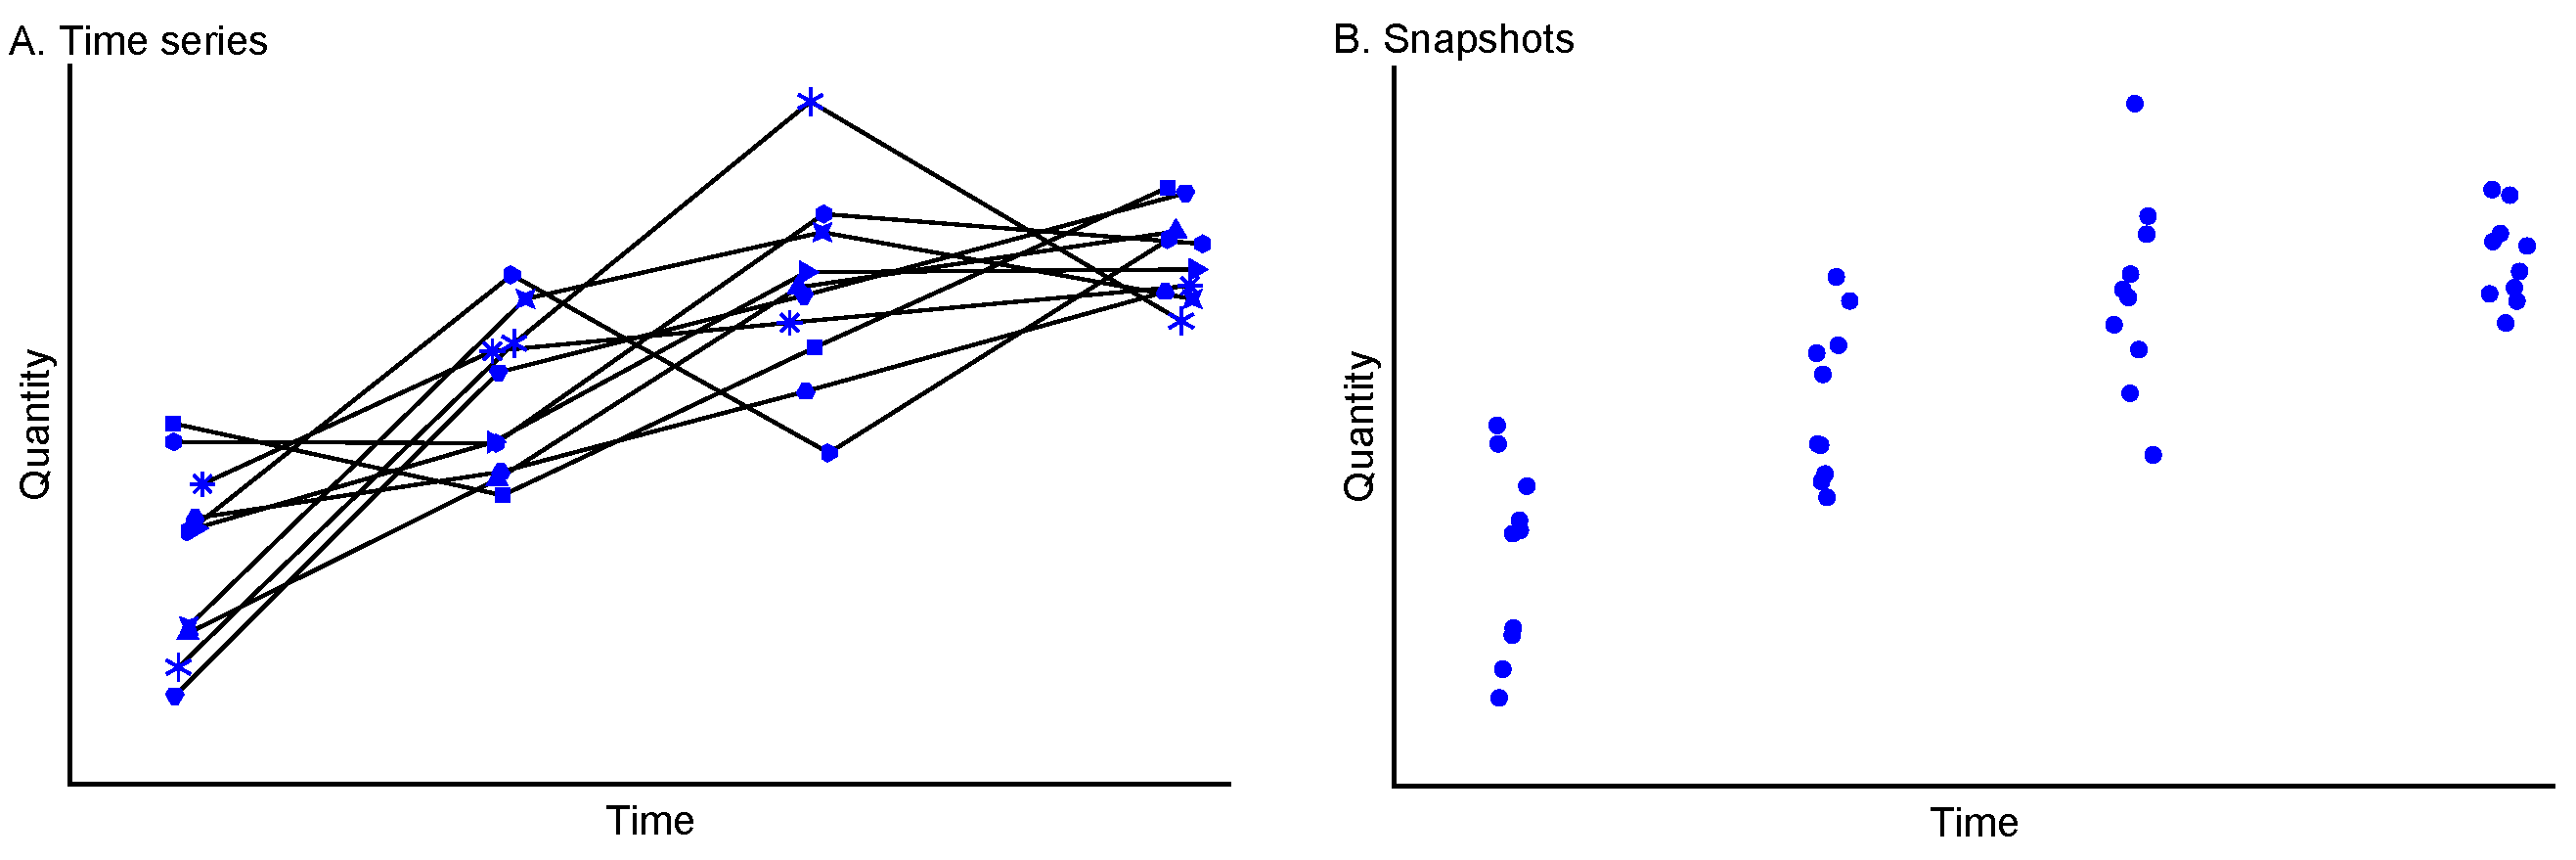
\includegraphics[width=\textwidth]{../figures/time_series_v_snapshots.pdf}}
	\caption{\textbf{Time series data (A) versus snapshot data (B) typical of single cell experiments.} In A that the cell identities are retained at each measurement point (indicated by given plot markers) whereas in the snapshot data in B, either this information is lost or, more often, cells are destroyed by the measurement process and so each observation corresponds to a distinct cell.}
	\label{fig:time_series_v_snapshots}
\end{figure}

We model the processes of an individual cell using a system of ordinary differential equations (ODEs), where each element of the system describes the governing dynamics of a particular quantity of interest (for example, protein levels, RNA concentrations and so on),
%
\begin{equation}\label{eq:ODE}
\dot{\boldsymbol{x}}(t) = f(\boldsymbol{x}(t); \boldsymbol{\theta}).
\end{equation}
%
Here $\boldsymbol{x}(t) = (x_1(t), x_2(t), ..., x_k(t))$ is a vector of states for each compartment in the system at time $t$ and $f(.)$ is a function of these states and parameters $\boldsymbol{\theta}\in\mathbb{R}^p$. Note that in most circumstances, the initial state of the system, $\boldsymbol{x}(0)$, is unknown and it is convenient to include these as elements of $\boldsymbol{\theta}$ to be estimated. The solution of eq. (\ref{eq:ODE}) is given by $\boldsymbol{x}(t) = g(t; \boldsymbol{\theta})$, where $\boldsymbol{x}(t)\in\mathbb{R}^k$ is a vector of outputs at time $t$ and $g(.)$ is a function that typically won't be analytically-determined; instead approximated via a numerical integration scheme. 

In this paper, we assume variation characterised by snapshot data arises due to between-cell heterogeneity in the underlying parameters $\theta$. Therefore, the evolution of the underlying state of cell $i$ is described by an idiosyncratic ODE,
%
\begin{equation}
\dot{\boldsymbol{x}^i}(t) = f(\boldsymbol{x}^i(t); \boldsymbol{\theta}^i),
\end{equation}
%
with solution $\boldsymbol{x}^i(t) = g(t; \boldsymbol{\theta}^i)$. The traditional (non-hierarchical) state-space approach to modelling dynamic systems supposes that measurement randomness generates output variation (Figure \ref{fig:data_generation}A). Our approach, by contrast, relies on the assumption that stochasticity in outputs is solely the result of variability in parameter values ($\boldsymbol{\theta}$) between cells (Figure \ref{fig:data_generation}B). Whether the assumption of ``perfect'' measurements is reasonable depends on the experimental details of  the system under investigation but we argue that our method nevertheless provides a useful approximation in many cases where the signal to noise ratio is high. 

\begin{figure}[H]
	\centerline{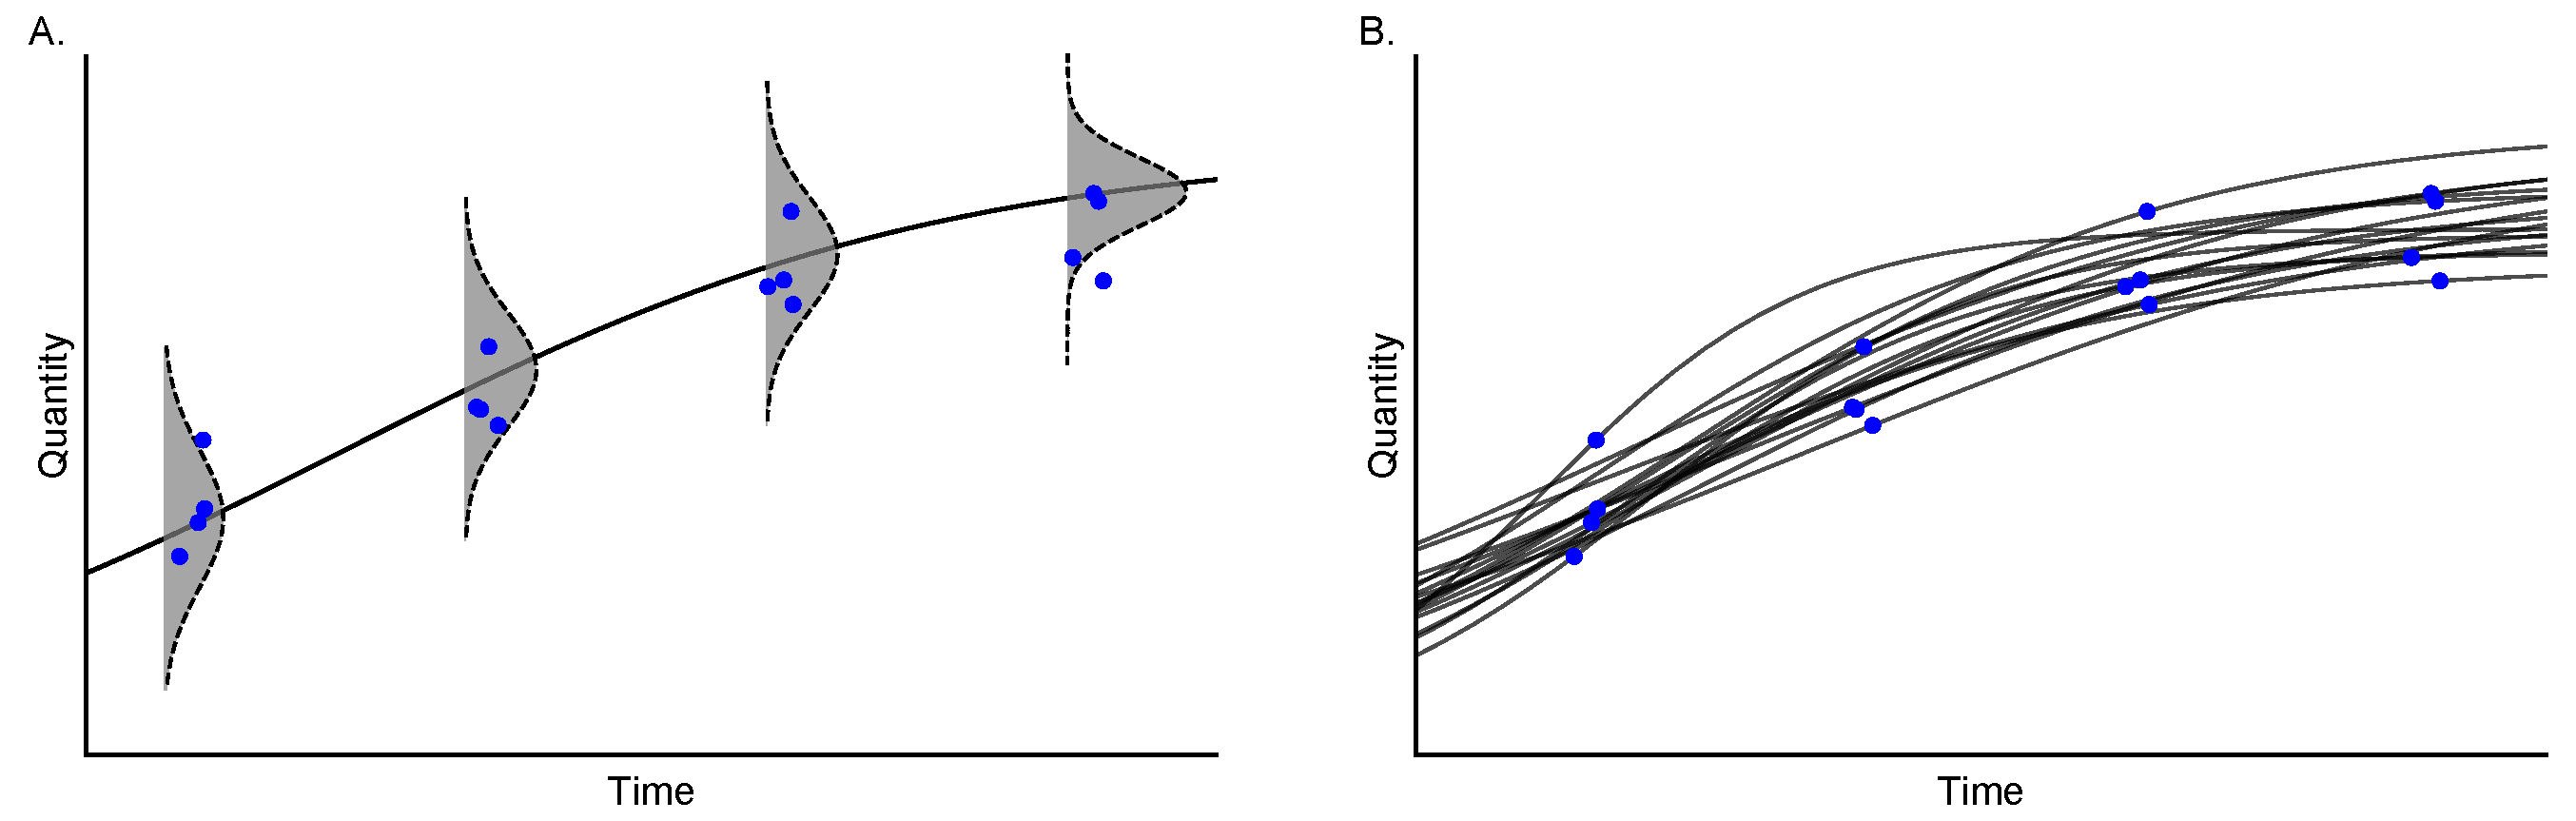
\includegraphics[width=\textwidth]{../figures/data_generation.pdf}}
	\caption{\textbf{Two ways to generate randomness in measured outputs: the state-space model (A) versus the parameter heterogeneity model (B).} For non-hierarchical state-space models (A), there is assumed to be a single ``true'' latent state where observations result from a noisy measurement process (grey histograms). For models with parameter heterogeneity (B), the uncertainty is generated by differences in cellular processes (black lines) between cells. Note that in both cases, individual cells are measured only once in their lifetime.}
	\label{fig:data_generation}
\end{figure}

Our generative model used to produce output observations for a single cell consists of two stages: (i) sample $\boldsymbol{\theta}^i\sim p(\boldsymbol{\theta})$, where $p(\boldsymbol{\theta})$ is a probability distribution characterising heterogeneity in cellular processes and, (ii) calculate output values using $\boldsymbol{x}_j^i(t') = g(t'; \boldsymbol{\theta})$ where, for each cell, a measurement of a subset $j$ of output states $\boldsymbol{x}_j^i(t')\in\boldsymbol{x}^i$ is made at a single point in time $t'\in (t_1, t_2, ..., t_o)$. The experimental observations for a single time point then consists of the collection of individual cell measurements $\boldsymbol{X}_j(t') = (\boldsymbol{x}_j^1(t'), \boldsymbol{x}_j^2(t'), ..., \boldsymbol{x}_j^n(t'))$, where $n$ is the number of cells measured at time $t'$. The entire observation dataset is the union of such sets across all measured time points $\boldsymbol{X}(\boldsymbol{t}) = (\boldsymbol{X}_{j_1}(t_1), \boldsymbol{X}_{j_2}(t_2), ..., \boldsymbol{X}_{j_o}(t_o))$, where $\boldsymbol{t}=(t_1, t_2, ..., t_o)$ is the vector of observation times and the subscript $a$ on each $j_a$ allows for measurement of different elements of the system at distinct timepoints.

\begin{table}[htbp]
	\centering
	\scriptsize
	\begin{adjustwidth}{-2in}{-1in}%
		\begin{tabularx}{1.65\textwidth}{lll}
			Variable	& Definition & Dimension\\
			\toprule
			$\boldsymbol{x}(t)$	& state of modelled system at time $t$ & $\mathbb{R}^k$\\
			$x_j(t)\in \boldsymbol{x}(t)$ & individual state $j$ of modelled system at time $t$ & $\mathbb{R}$\\
			$\boldsymbol{\theta}$ & parameters of ODE system & $\mathbb{R}^p$\\
			$f(\boldsymbol{x}(t); \boldsymbol{\theta})$	& function specifying RHS of ODE system & $\mathbb{R}^k$\\
			$g(t; \boldsymbol{\theta})$	&  solution of ODE at time $t$ & $\mathbb{R}^k$\\
			$g_j(t; \boldsymbol{\theta})$	&  solution of ODE for state $j$ at time $t$ & $\mathbb{R}$\\
			$\boldsymbol{x}^i(t)$ &  state of modelled system of cell $i$ at time $t$ & $\mathbb{R}^k$\\
			$\boldsymbol{x}_j^i(t)\in\boldsymbol{x}^i(t)$ & state of subset $j$ of modelled system of cell $i$ at time $t$ & $\mathbb{R}^{|j|}$ \\
			$\boldsymbol{X}_j(t)=(\boldsymbol{x}^1_j(t),...,\boldsymbol{x}^n_j(t))$ & collection of $n$ individual cell measurements at time $t$ & $\mathbb{R}^{|j|\times n}$\\
			$\boldsymbol{t}=(t_1, t_2, ..., t_o)$ & unique observation times & $\mathbb{R}^o$\\
			$\boldsymbol{X}(\boldsymbol{t})=(\boldsymbol{X}_{j_1}(t_1), ..., \boldsymbol{X}_{j_o}(t_o))$ & all observations collected at times $\boldsymbol{t}$ & $\text{dim}(\boldsymbol{X}_{j_1}) \times ... \times \text{dim}(\boldsymbol{X}_{j_o})$\\
			$\Phi$ & parameters characterising output target distribution $p(\boldsymbol{x}|\Phi)$ & -\\
			$\hat{a}$ & estimates of any quantity $a$ & -\\
			$\tilde{\boldsymbol{t}}=(t_1,...,t_m)$ & times when each observable is recorded & $\mathbb{R}^m$\\
			$\tilde{\boldsymbol{x}}(\tilde{\boldsymbol{t}})=(x_{j_1}(t_1), ..., x_{j_m}(t_m))$ & system observables & $\mathbb{R}^m$\\
			$\mathcal{V}(\tilde{\boldsymbol{x}})$ & the ``volume'' of parameter space mapping to an output of value $\boldsymbol{x}$ &  $\mathbb{R}^+$\\
			$\boldsymbol{g}(\boldsymbol{\theta})=\boldsymbol{g}(\tilde{\boldsymbol{t}};\boldsymbol{\theta})=(g_{j_1}(t_1; \boldsymbol{\theta}),...,g_{j_m}(t_m; \boldsymbol{\theta}))$ & solution of ODE for each observable at respective times $\boldsymbol{t}$ & $\mathbb{R}^m$\\
			$V$ & total volume of parameter space with uniform priors used for all parameters & $\mathbb{R}^+$\\
			$\Omega(\tilde{\boldsymbol{x}}) = \{\boldsymbol{\theta}: \boldsymbol{g}(\boldsymbol{\theta}) = \tilde{\boldsymbol{x}}\}$ & region of parameter space mapping to output $\tilde{\boldsymbol{x}}$ & $\mathbb{R}^p$\\
			$\Psi$ & parameters characterising output prior distribution $p(\tilde{\boldsymbol{x}}|\Psi)$ & -\\
			$\Xi$ & parameters characterising parameter prior distribution $p(\boldsymbol{\theta}|\Xi)$ & -
			\end{tabularx}
		\caption{\textbf{Glossary of variable names used in this paper.} The dimensions of $\Phi$, $\Psi$ and $\Xi$ are listed as ``-'' since they depend on the form of the density used to represent the process and can be anywhere from $\mathbb{R}^1$ to $\mathbb{R}^\infty$. The variables are listed in the approximate order in which they appear in the text.}
		\label{tab:variable_glossary}%
	\end{adjustwidth}
\end{table}%

Raw snapshot data consists of measurements of individual cells with exact inference requiring simulating the underlying ODE system for each individual. This is cumbersome and impractical for the numbers of cells sampled in typical experimental setups and so, instead, we follow previous work and instead represent snapshot data using probability distributions \cite{hasenauer2011identification,hasenauer2014ode,loos2018hierarchical,dixit2018maximum}. The snapshots themselves can either be distributions of a single species or multiple species, which can be approximated by univariate and multivariate probability distributions respectively. These probability distributions are characterised by parameter estimates $\hat{\Phi}$ determined by the output observations $\boldsymbol{X}(\boldsymbol{t})$. The dimensionality of these probability distributions depends on the set of $m$ distinct observables $\tilde{\boldsymbol{x}}(\tilde{\boldsymbol{t}})=(x_{j_1}(t_1), x_{j_2}(t_2), ..., x_{j_m}(t_m))$ recorded by experimental measurements. Note that, $\tilde{\boldsymbol{x}}(\tilde{\boldsymbol{t}})$ corresponds to a particular set of measurements from a hypothetical cell and is distinct from $\boldsymbol{X}(\boldsymbol{t})$, which represents the full set of experimental outputs. The vector $\tilde{\boldsymbol{x}}(\tilde{\boldsymbol{t}})$ is hypothetical because in reality each cell is measured at a single timepoint (although we suppose measurements of different cellular attributes are possible contemporaneously).

The goal of our inference process is to  characterise the probability distribution $p(\boldsymbol{\theta}|\boldsymbol{X}(\boldsymbol{t}))$ representing heterogeneity in cellular processes. The first step in our inference workflow is to fit the output distributions using probability distributions (Figure \ref{fig:workflow}(i)). We assume that the volume of observational data means the estimated probability distributions are approximate sufficient statistics of the outputs, meaning $p(\boldsymbol{\theta}|\hat{\Phi}) \approx p(\boldsymbol{\theta}|\boldsymbol{X}(\boldsymbol{t}))$.

\begin{figure}[H]
	\centerline{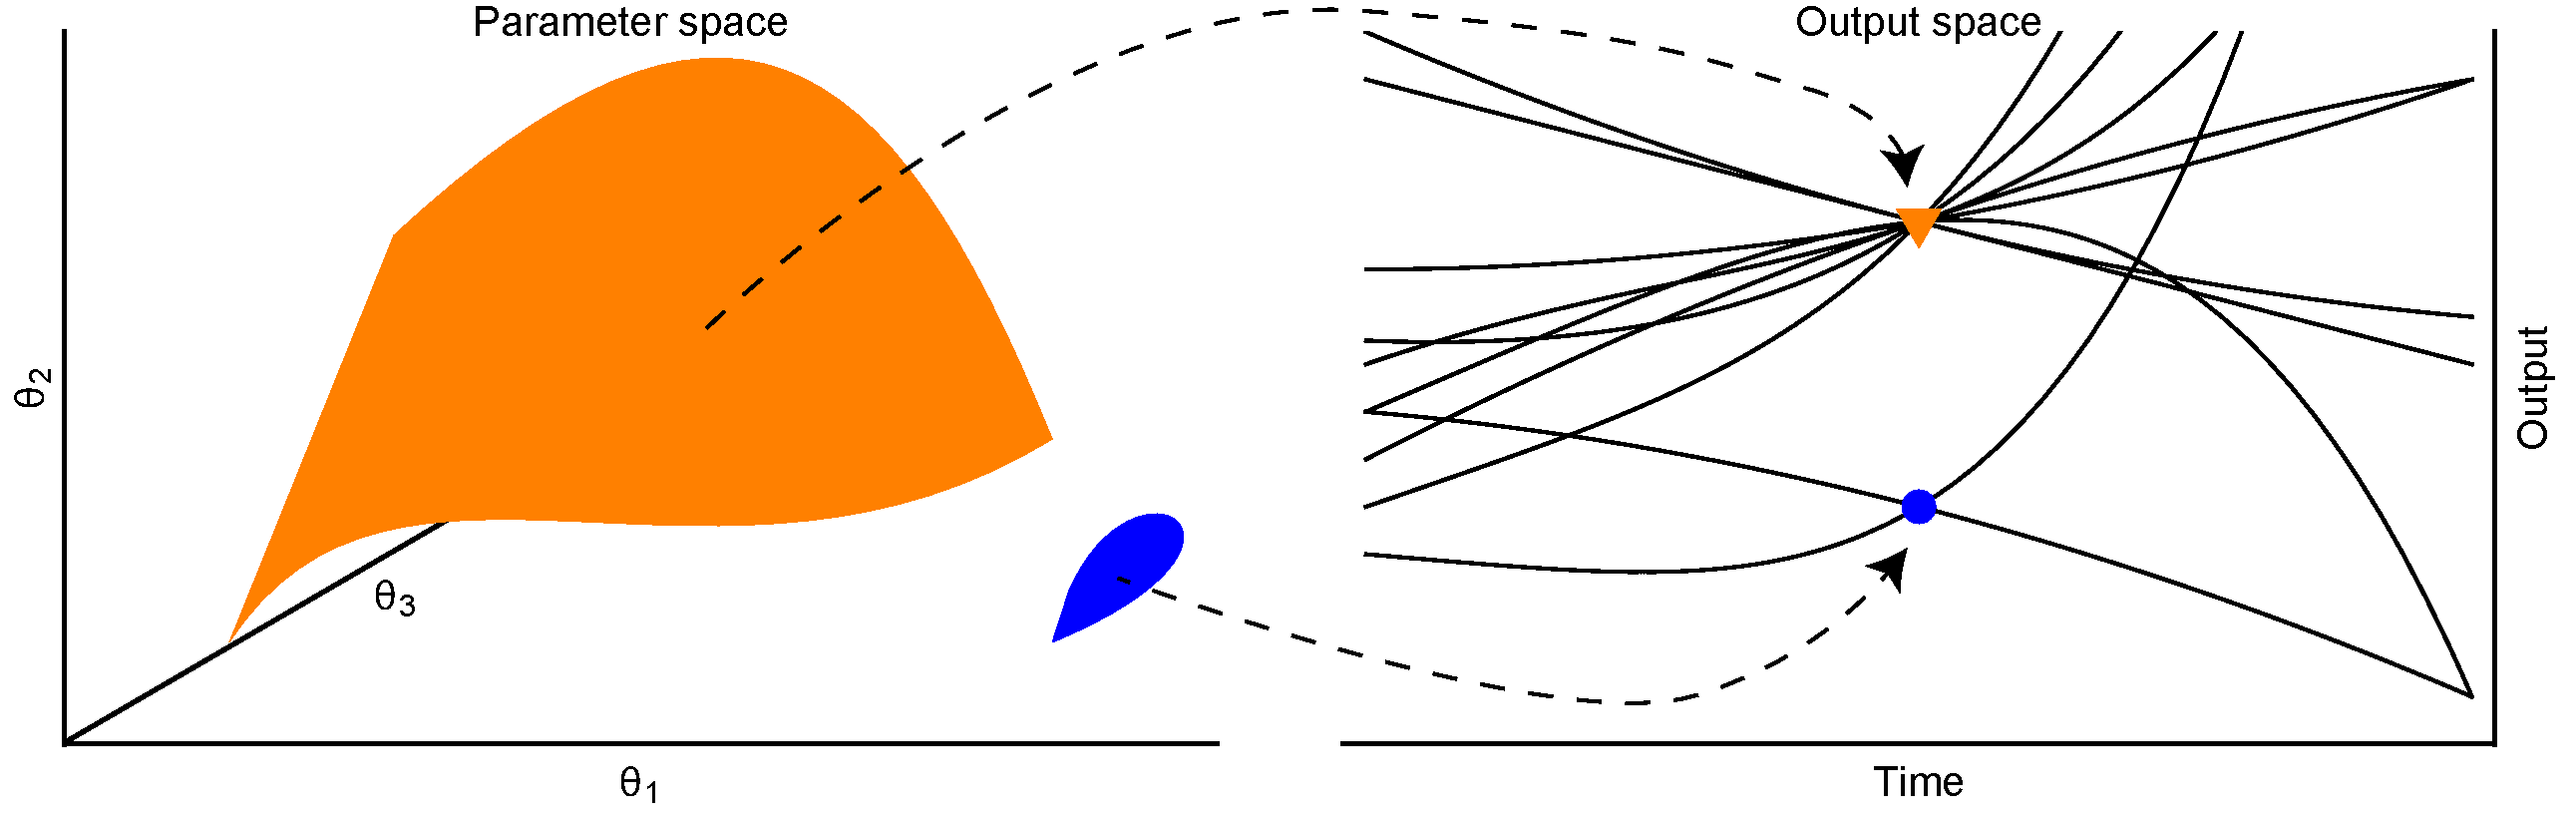
\includegraphics[width=\textwidth]{../figures/contour_volumes.pdf}}
	\caption{\textbf{The non-linear mapping from parameter values (left panel) to outputs (black lines; right panel) means different sized regions of parameter space (orange and blue surfaces; left panel) correspond to distinct output values (orange triangle and blue square; right panel).} In the right panel, each black line represents a distinct model simulation $g(t; \theta_1, \theta_2, \theta_3)$ and the triangle and square indicate outputs at a given point in time.}
	\label{fig:contour_volumes}
\end{figure}


The models we seek to fit to snapshot data mostly cannot be identified from the observations. This is often because the number of model parameters exceeds the dimensionality of the output distribution (that is, $m>k$) meaning there typically exist non-singular sets of parameter values mapping to a single set of output values. That is, each vector of observed outputs $\tilde{\boldsymbol{x}}\in\mathbb{R}^m$, can often be caused by many combinations of parameters although, due to the non-linearity of the map from parameters to outputs, the ``volume'' of these regions of parameter space, $\mathcal{V}(\tilde{\boldsymbol{x}})$, is a function of output (Figure \ref{fig:contour_volumes}). In what follows, we make clear the distinction between observables $\tilde{\boldsymbol{x}}(\tilde{\boldsymbol{t}})$ and the vector-valued function representing modelled outputs $\boldsymbol{g}(\tilde{\boldsymbol{t}}; \boldsymbol{\theta})=(g_{j_1}(t_1; \boldsymbol{\theta}),g_{j_2}(t_2; \boldsymbol{\theta}),...,g_{j_m}(t_m; \boldsymbol{\theta}))\in\mathbb{R}^m$ since the latter is a function whereas that latter is a numeric value; we also drop the $\tilde{\boldsymbol{t}}$ notation from following expressions to minimise clutter.

A consequence of this non-linear parameter to output geometry is that any target output distribution $p(\tilde{\boldsymbol{x}}|\hat{\Phi})$ does not correspond to a unique parameter distribution. For example, suppose $g(\theta_1, \theta_2) = \theta_1 + \theta_2$: the target distribution $\tilde{\boldsymbol{x}}\sim \mathcal{N}(0, 1)$ can be generated by any member of the set of parameter distributions $\sqrt{\eta} \theta_1 + \sqrt{1 - \eta} \theta_2$, where $\eta\in [0, 1]$ and $\theta_1, \theta_2 \sim \mathcal{N}(0, 1)$. This means that in order to ensure uniqueness of the ``posterior'' parameter distributions, we are required to specify ``prior'' distributions for the parameters, as in more traditional Bayesian inference. An additional consequence of the degeneracy of the mapping from parameters to outputs is that any sampling algorithm aimed at exploring posterior parameter space must account for the differential volumes of iso-output contours. Whilst we refer the interested reader to our companion paper on this subject [citation for tutorial paper published in Open Science], we provide a quick derivation of the posterior parameter distribution which accounts for the non-linear mapping.

To derive the posterior distribution of parameter values $p(\boldsymbol{\theta}|\hat{\Phi})$, we consider the joint density of parameters and outputs $p(\boldsymbol{\theta},\tilde{\boldsymbol{x}}|\hat{\Phi})$. This can be decomposed in two ways, 
%
\begin{equation}\label{eq:joint}
p(\boldsymbol{\theta}|\tilde{\boldsymbol{x}}, \hat{\Phi}) \times p(\tilde{\boldsymbol{x}}|\hat{\Phi}) = p(\boldsymbol{\theta},\tilde{\boldsymbol{x}}|\hat{\Phi}) =  p(\tilde{\boldsymbol{x}}| \boldsymbol{\theta}, \hat{\Phi}) \times p(\boldsymbol{\theta}|\hat{\Phi}).
\end{equation}
%
The left and right hand sides of eq. (\ref{eq:joint}) can be equated and rearranged to obtain the posterior parameter distribution,
%
\begin{equation}
p(\boldsymbol{\theta}|\hat{\Phi}) = \frac{p(\boldsymbol{\theta}|\tilde{\boldsymbol{x}}, \hat{\Phi}) \times p(\tilde{\boldsymbol{x}}|\hat{\Phi})}{p(\tilde{\boldsymbol{x}}| \boldsymbol{\theta}, \hat{\Phi})}.
\end{equation}
%
Given parameters $\boldsymbol{\theta}$, the mapping from parameters to outputs is deterministic meaning $p(\tilde{\boldsymbol{x}}| \boldsymbol{\theta}, \hat{\Phi})=\delta(\boldsymbol{g}(\boldsymbol{\theta}))$ is the Dirac delta function centred at $\tilde{\boldsymbol{x}}=\boldsymbol{g}(\boldsymbol{\theta})$. In what follows, we assume that the conditional distribution $p(\boldsymbol{\theta}|\tilde{\boldsymbol{x}}, \hat{\Phi})$ is independent of the data, meaning it represents a conditional ``prior'', which can be manipulated by Bayes' rule,
%
\begin{equation}\label{eq:prior}
p(\boldsymbol{\theta}|\boldsymbol{g}(\boldsymbol{\theta})) = \frac{p(\boldsymbol{\theta})}{p(\boldsymbol{g}(\boldsymbol{\theta}))},
\end{equation}
%
where we have used the Dirac delta function for $p(\tilde{\boldsymbol{x}}|\boldsymbol{\theta})$. This results in the form of the posterior parameter distribution targeted by our sampling algorithm,
%
\begin{equation}\label{eq:posterior_input}
p(\boldsymbol{\theta}|\hat{\Phi}) = \frac{p(\boldsymbol{\theta})}{p(\boldsymbol{g}(\boldsymbol{\theta}))} p(\boldsymbol{g}(\boldsymbol{\theta})|\hat{\Phi}).
\end{equation}
%
Again, we refer to our companion piece [citation] for detailed explanation of eqs. (\ref{eq:prior}) \& (\ref{eq:posterior_input}) and instead here provide brief interpretation when considering a uniform prior on parameter space. In this case, $p(\boldsymbol{\theta}) = \frac{1}{V}$, where $V$ is the total volume of parameter space. The denominator term of eq. (\ref{eq:prior}) is the prior induced on output space by the prior over parameter space. For a uniform prior on parameter values, this is just proportion of parameter space where $\boldsymbol{g}(\boldsymbol{\theta}) = \tilde{\boldsymbol{x}}$, meaning,
%
\begin{equation}\label{eq:contour_volume}
p(\boldsymbol{\theta}|\boldsymbol{g}(\boldsymbol{\theta})) = \frac{1}{\mathcal{V}(\boldsymbol{g}(\boldsymbol{\theta}))},
\end{equation}
%
where $\mathcal{V}(\boldsymbol{g}(\boldsymbol{\theta}))$ is the volume of parameter space occupied by the iso-output region $\Omega(\tilde{\boldsymbol{x}}) = \{\boldsymbol{\theta}: \boldsymbol{g}(\boldsymbol{\theta}) = \tilde{\boldsymbol{x}}\}$. Therefore a uniform prior over parameter space implies a prior structure where all  parameter values resulting in the same output $\tilde{\boldsymbol{x}}$ are given equal weighting.

The denominator term of eq. (\ref{eq:prior}) cannot be calculated apart from for some toy examples, meaning that exact sampling from the posterior parameter distribution of eq. (\ref{eq:posterior_input}) is not, in general, possible. We propose instead a computationally efficient sampling method to estimate $p(\boldsymbol{g}(\boldsymbol{\theta}))$, which forms the first step of our so-called ``Contour Monte Carlo'' (CMC) algorithm (Algorithm \ref{alg:cmc}; Figure \ref{fig:workflow}(ii)), where we estimate the volume of iso-output contours with output value $\boldsymbol{g}(\boldsymbol{\theta})$. This step involves repeated independent sampling from the prior distribution of parameters $\boldsymbol{\theta}^i\sim p(\boldsymbol{\theta}|\Xi)$, where, for completeness, we have conditioned on $\Xi$ parameterising our probability density. Each parameter sample is then converted into an output value $\tilde{\boldsymbol{x}}^i=\boldsymbol{g}(\boldsymbol{\theta}^i)$. The collection of output samples is then fitted using a vine copula kernel density estimator (KDE) \cite{nagler2016evading}, $(\tilde{\boldsymbol{x}}^1,\tilde{\boldsymbol{x}}^2,...,\tilde{\boldsymbol{x}}^{N_1})\sim p(\tilde{\boldsymbol{x}}|\hat{\Psi})$. Throughout the course of development of CMC, we have tested many forms of KDE and have found vine copula KDE is best suited to approximating the higher dimensional probability distributions required in practice.

The second step in our algorithm then uses Markov chain Monte Carlo (MCMC) to sample from an approximate version of eq. (\ref{eq:posterior_input}) with the estimated density $p(\boldsymbol{g}(\boldsymbol{\theta})|\hat{\Psi})$ replacing its corresponding estimand (Algorithm \ref{alg:cmc}; Figure \ref{fig:workflow}(iii)),
%
\begin{equation}\label{eq:posterior_input_estimated}
p(\boldsymbol{\theta}|\hat{\Phi},\Xi,\hat{\Psi}) = \frac{p(\boldsymbol{\theta}|\Xi)}{p(\boldsymbol{g}(\boldsymbol{\theta})|\hat{\Psi})} p(\boldsymbol{g}(\boldsymbol{\theta})|\hat{\Phi}).
\end{equation}
%

\begin{algorithm}[H]
	\footnotesize
	\texttt{\\}
	\begin{algorithmic}
		\Procedure{CMC}{$\boldsymbol{X}(\boldsymbol{t}), \Xi, N_1, N_2$}\Comment{Sample from posterior parameter distribution}
		\State $\hat{\Phi} = \Call{SnapshotEstimator}{\boldsymbol{X}(\boldsymbol{t})}$
		\State $\hat{\Psi} = \Call{ContourVolumeEstimator}{\Xi}$
		\State $(\boldsymbol{\theta}_1,...,\boldsymbol{\theta}_{N_2}) = \Call{MCMC}{\hat{\Phi},\Xi, \hat{\Psi}}$
		\State $\text{converged} = \Call{CompareOutputToTarget}{(\boldsymbol{\theta}_1,...,\boldsymbol{\theta}_{N_2}), \hat{\Psi}}$
		\If{converged$\neq$1}
		\State $(\boldsymbol{\theta}_1,...,\boldsymbol{\theta}_{N_2})$=\Call{ContourVolumeEstimator}{$\hat{\Phi}, \Xi, N_1', N_2'$}
		\State where, $N_1' > N_1$ and/or $N_2' > N_2$ \Comment{Rerun contour volume estimation and/or MCMC with larger sample sizes}
		\EndIf
		\State \Return $(\boldsymbol{\theta}_1,...,\boldsymbol{\theta}_{N_2})$
		\EndProcedure
	\end{algorithmic}

	\texttt{\\}
	\begin{algorithmic}
		\Procedure{SnapshotEstimator}{$\boldsymbol{X}(\boldsymbol{t})$}\Comment{Fit density to snapshot observations}
		\State $\boldsymbol{X}(\boldsymbol{t}) \sim p(\tilde{\boldsymbol{x}}|\hat{\Phi})$
		\State \Return $\hat{\Phi}$
		\EndProcedure
	\end{algorithmic}
	
	\texttt{\\}
	\begin{algorithmic}
		\Procedure{ContourVolumeEstimator}{$ \Xi$}\Comment{Estimate volume of contours}
		\For{$i$ in $1:N_1$}
		\State $\boldsymbol{\theta}_i\sim p(\boldsymbol{\theta}|\Xi)$ \Comment{Sample from prior density}
		\State $\tilde{\boldsymbol{x}}_i = \boldsymbol{g}(\boldsymbol{\theta}_i)$ \Comment{Calculate corresponding output value}
		\EndFor
		\State $(\tilde{\boldsymbol{x}}_1,\tilde{\boldsymbol{x}}_2,...,\tilde{\boldsymbol{x}}_{N_1}) \sim p(\tilde{\boldsymbol{x}}|\hat{\Psi})$ \Comment{Fit vine copula kernel density estimator to output values.}
		\State \Return $\hat{\Psi}$
		\EndProcedure
	\end{algorithmic}

	\texttt{\\}
	\begin{algorithmic}
		\Procedure{MCMC}{$\hat{\Phi},\Xi, \hat{\Psi}$}\Comment{Random Walk Metropolis algorithm targeting posterior parameter distribution.}
		\State $\boldsymbol{\theta}_0 \sim \pi(.)$ \Comment{Sample from arbitrary initialisation distribution}
		\For{$i$ in $1:N_2$}
		\State $\boldsymbol{\theta}_i'\sim \mathcal{N}(\boldsymbol{\theta}_{i-1},\boldsymbol{\Sigma})$ \Comment{Propose new parameter values for parameters}
		\State $r = \left[p(\boldsymbol{\theta}'|\Xi) p(\boldsymbol{g}(\boldsymbol{\theta})|\hat{\Psi})p(\boldsymbol{g}(\boldsymbol{\theta}')|\hat{\Phi})\right] / \left[p(\boldsymbol{\theta}|\Xi) p(\boldsymbol{g}(\boldsymbol{\theta}')|\hat{\Psi})p(\boldsymbol{g}(\boldsymbol{\theta})|\hat{\Phi})\right]$\Comment{Metropolis acceptance ratio.}
		\State $u\sim U(0,1)$ \Comment{Sample from uniform distribution}
		\If{$r > u$}
		\State $\boldsymbol{\theta}_i = \boldsymbol{\theta}_i'$ \Comment{Accept proposal}
		\Else
		\State $\boldsymbol{\theta}_i = \boldsymbol{\theta}_{i-1}$ \Comment{Reject proposal}
		\EndIf
		\EndFor
		\State \Return $(\boldsymbol{\theta}_1,...,\boldsymbol{\theta}_{N_2})$
		\EndProcedure
	\end{algorithmic}

	\texttt{\\}
	\begin{algorithmic}
			\Procedure{CompareOutputToTarget}{$(\boldsymbol{\theta}_1,...,\boldsymbol{\theta}_{N_2}), \hat{\Psi}$}\Comment{Check output distribution close to target}
		\For{$i$ in $1:N_2$}
		\State $\tilde{\boldsymbol{x}}_i = \boldsymbol{g}(\boldsymbol{\theta}_i)$ \Comment{Compute output for each parameter sample}
		\EndFor
		\If{$(\tilde{\boldsymbol{x}}_1,\tilde{\boldsymbol{x}}_2,...,\tilde{\boldsymbol{x}}_{N_2})\sim p(\tilde{\boldsymbol{x}}|\hat{\Psi})?$} \Comment{Compare outputs with target}
		\State \Return 1 \Comment{If outputs sufficiently close then converged}
		\Else
		\State \Return 0
		\EndIf
		\EndProcedure
	\end{algorithmic}

	\caption{Pseudocode for the Contour Monte Carlo algorithm for sampling from the posterior parameter distribution of eq. (\ref{eq:posterior_input_estimated}). Here we provide code for the Random Walk Metropolis algorithm for the MCMC sampling but for the examples in \S \ref{sec:results}, we use an adaptive MCMC algorithm \cite{johnstone2016uncertainty}. A definition of all variables is provided in Table \ref{tab:variable_glossary}.}\label{alg:cmc}
\end{algorithm}

\begin{figure}[H]
	\centerline{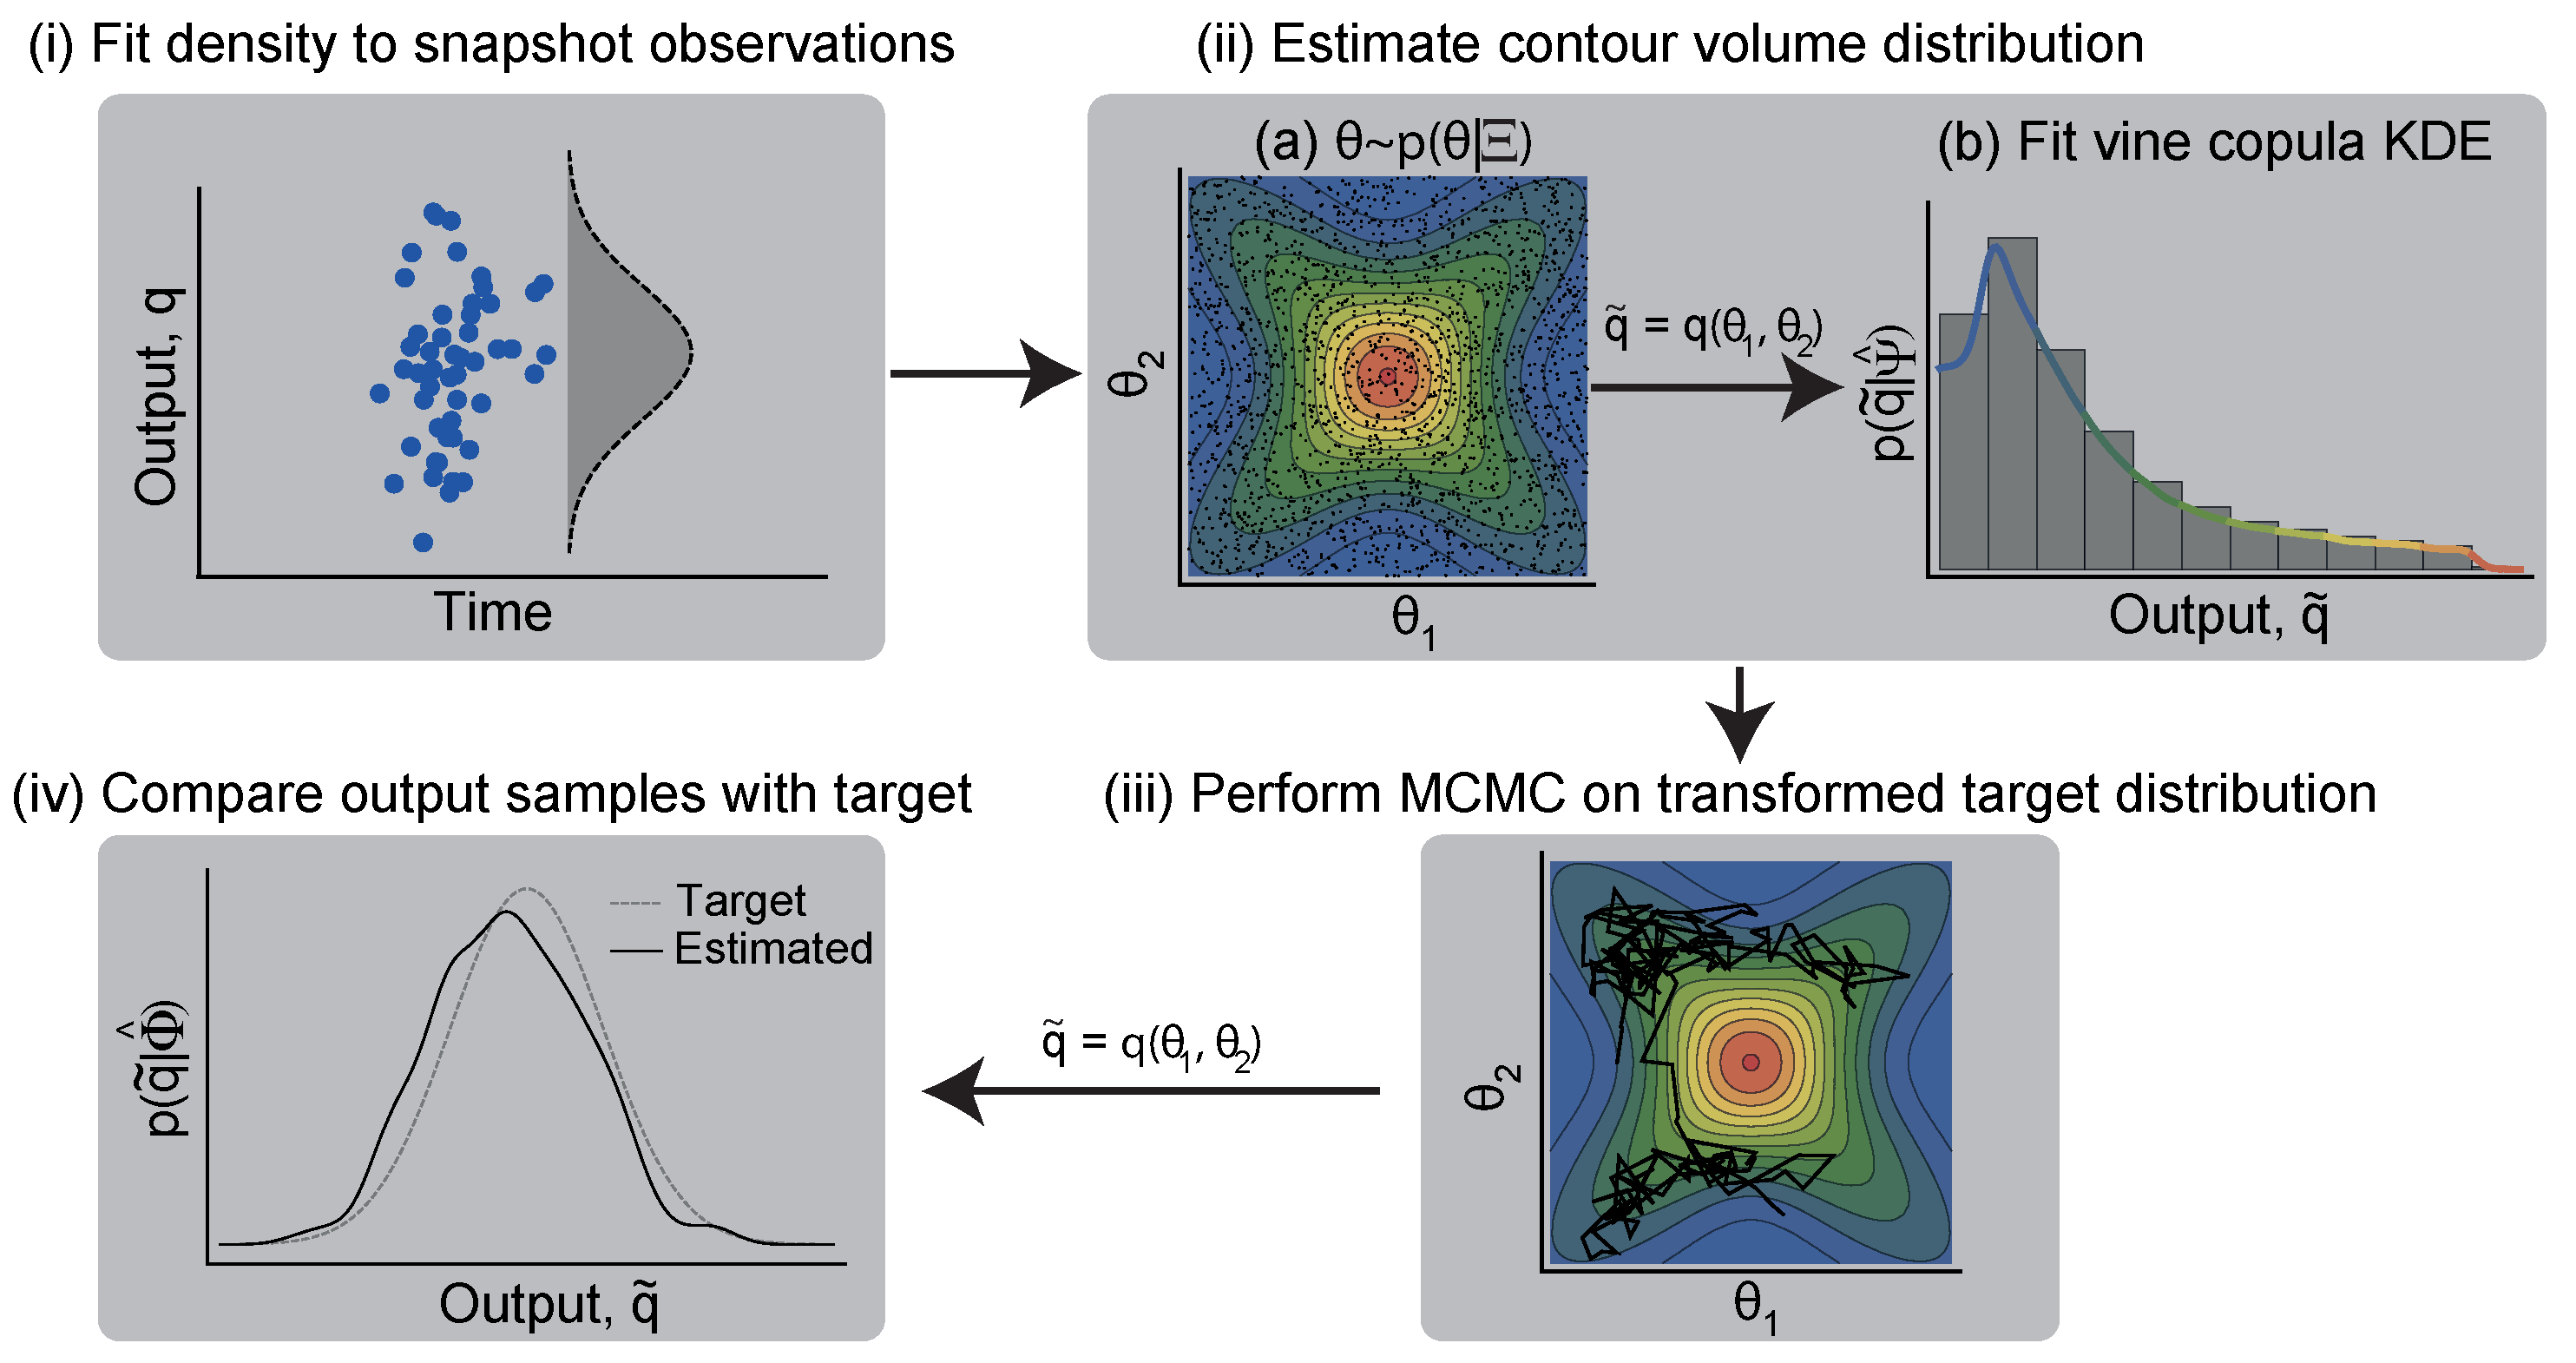
\includegraphics[width=\textwidth]{../figures/workflow.pdf}}
	\caption{\textbf{The workflow for using Contour Monte Carlo to estimate cell population heterogeneity.} In (iii), the distribution targeted is given by eq. (\ref{eq:posterior_input_estimated}) but with $p(\tilde{\boldsymbol{x}}|\hat{\Psi})\rightarrow p(g(\boldsymbol{\theta}))$. The variables used in this figure are defined in the text and Table \ref{tab:variable_glossary}.}
	\label{fig:workflow}
\end{figure}

The final step in CMC is to transform parameter samples from the MCMC into outputs, then compare the sampled outputs with the target distribution (Figure \ref{fig:workflow}(iv)). Asymptotically (in terms of the sample size of both sampling steps), CMC produces a sample of parameter values $(\boldsymbol{\theta}^1,\boldsymbol{\theta}^2,...)$ which, when transformed to outputs, corresponds to the target distribution $p(\boldsymbol{x}|\hat{\Psi})$. In developing CMC, we have found that a finite sample of modest size for both steps of CMC results in parameter samples that, when transformed, often represent reasonable approximations of the target. There are however occasions when this is not the case and we have found this final confirmatory step indispensable since it frequently highlights inadequacies in the contour volume estimation or the MCMC, meaning more samples from either or both of these steps are required. It may also be necessary to tweak hyperparameters of the KDE to ensure reasonable approximation in the contour volume estimation step. If the target distribution is sensitive to the contour volume estimates, this may also indicate that the target snapshot distribution is incompatible with the model: here, we make no claims on existence of a solution to the inverse problem, only that, if one should exist, Contour Monte Carlo is a pragmatic approach to approximate it by sampling. A useful way to diagnose whether the target distribution can be produced from the model and specified priors is to examine the output values from the contour volume estimation step of CMC. If the majority of probability mass of the target lies outside the bounds of the bulk simulated output values obtained by independent sampling from the prior, then the model and/or chosen prior is unlikely to be invertible to this particular target. 

For the contour volume estimation step, we assumed sample sizes were sufficient if the output samples from the MCMC provided a reasonable approximation to the target, although we recognise that future work should refine this process further. For the MCMC step, we use adaptive covariance MCMC (see SOM of \cite{johnstone2016uncertainty}) to sample from the target distribution, as we have found that it provides a considerable speed-up over Random Walk Metropolis \cite{metropolis1953equation,lambert2018Student}. We also use the Gelman-Rubin convergence statistic $\hat{R}$ which provides a heuristic measurement of convergence \cite{lambert2018Student,gelman1992inference}, and use a threshold of $\hat{R}\leq\sim 1.1$ to diagnose convergence.


\section{Results}\label{sec:results}
In this section, we use CMC to estimate the posterior parameter distribution for three biological systems of interest targeting synthetic parametric densities. That is, we assume that the first step of CMC (``SnapshotEstimator'' within Algorithm \ref{alg:cmc}) has already been undertaken and we are faced with inferring a parameter distribution which, when transformed to outputs, recapitulates the target density. Alongside the text, we also provide a Julia notebook used to generate the results, which we hope will be of use to others wanting to apply CMC to estimate cell population heterogeneity.


\begin{table}[htbp]
	\centering
	\scriptsize
	\begin{adjustwidth}{-1.0in}{-0.1in}%
		\begin{tabularx}{1.4\textwidth}{llllll}
			Model	& Target density & Parameter & Prior density & Prior parameter 1 & Prior parameter 2\\
			\toprule
			Growth factor & two-dimensional normal & $R_T$ & uniform & $2.5 \times 10^5$ &  $8 \times 10^5$\\
			&& $k_1$ & uniform & 0.25 & 3.0\\
			&& $k_{-1}$ & uniform & 2.0 & 20.0\\
			&& $k_{deg}$ & uniform & 0.005 & 0.03\\
			&& $k^*_{deg}$ & uniform & 0.1 & 0.5\\
			\toprule
			Growth factor & two-dimensional normal & $R_T$ & normal & $5 \times 10^5$ &  $1 \times 10^5$\\
			&& $k_1$ & normal & 0.5 & 0.1\\
			&& $k_{-1}$ & normal & 3.0 & 1.0\\
			&& $k_{deg}$ & normal & 0.02 & 0.005\\
			&& $k^*_{deg}$ & normal & 0.3 & 0.1\\
			\toprule
			Michaelis-Menten kinetics & bimodal normal & $k_f$ & uniform & 0.2 &  15\\
			&& $k_r$ & uniform & 0.2 & 2.0\\
			&& $k_{cat}$ & uniform & 0.5 & 3.0\\
			\toprule
			Michaelis-Menten kinetics & four-dimensional normal & $k_f$ & uniform & 0.2 &  15\\
			&& $k_r$ & uniform & 0.2 & 2.0\\
			&& $k_{cat}$ & uniform & 0.2 & 3.0\\
			&& $E_0$ & uniform & 3.0 & 5.0\\
			&& $S_0$ & uniform & 5.0 & 10.0\\
			&& $ES_0$ & uniform & 0.0 & 0.2\\
			&& $P_0$ & uniform & 0.0 & 0.2\\
			\toprule
			TNF signalling & bimodal normal & $a_1$ & uniform & 0.5 & 0.7\\
			&& $a_2$ & uniform & 0.1 & 0.3\\
			&& $a_3$ & uniform & 0.1 & 0.3\\
			&& $a_4$ & uniform & 0.4 & 0.6\\
			&& $b_1$ & uniform & 0.3 & 0.5\\
			&& $b_2$ & uniform & 0.6 & 0.8\\
			&& $b_3$ & uniform & 0.2 & 0.4\\
			&& $b_4$ & uniform & 0.4 & 0.6\\
			&& $b_5$ & uniform & 0.3 & 0.5\\
		\end{tabularx}
	\caption{\textbf{The priors used for each problem in \S\ref{sec:results}.}}
	\label{tab:priors}
	\end{adjustwidth}
\end{table}

\subsection{Growth factor model}
Here we consider the ``growth factor model'' introduced by \cite{dixit2018maximum}, which concerns the dynamics of inactive ligand-free cell surface receptors $R$ and active ligand-bound cell surface receptors $P$, modulated by an exogenous ligand $L$. The governing dynamics are determined by the following system,
%
\begin{align}\label{eq:growth_factor}
\frac{\mathrm{d}R}{\mathrm{d}t} &= R_T k_{deg} + k_1 L R + k_{-1} P - k_{deg} R\\
\frac{\mathrm{d}P}{\mathrm{d}t} &= k_1 L R - k_{-1} P - k^*_{deg} P,
\end{align}
%
where $\boldsymbol{\theta}=(R_T, k_1, k_{-1}, k_{deg}, k^*_{deg})$ are parameters to be determined. In this example, we use measurements of the active ligand-bound receptors $P$ to estimate cellular heterogeneity in processes. We denote the solution of eq. (\ref{eq:growth_factor}) as $P(t; \boldsymbol{\theta}, L)$ and seek to determine the parameter distribution consistent with an output distribution,
%
\begin{equation}\label{eq:MM_outputDistribution}
\begin{pmatrix}
P(10; \boldsymbol{\theta}, 2)\\
P(10; \boldsymbol{\theta}, 10)\\
\end{pmatrix} \sim  \mathcal{N}
\begin{bmatrix}
\begin{pmatrix}
2\times 10^4\\
3\times 10^4\\
\end{pmatrix}, \;\;
\begin{pmatrix}
1\times 10^5 & 0\\
0 & 1\times 10^5\\
\end{pmatrix}
\end{bmatrix}.
\end{equation}
%
To start, we specify a uniform prior for each of the five parameters, with bounds given in Table \ref{tab:priors}. To estimate the posterior parameter distribution, we use CMC, with adaptive covariance MCMC \cite{johnstone2016uncertainty} for the second step.

In Figure \ref{fig:growth_factor_outputs}A, we show the target distributions of outputs (black solid lines and contours) versus the sampled distribution (blue dots and dashed lines), illustrating that CMC is able to recapitulate the target densities using modest sample sizes. In Figure \ref{fig:growth_factor_inputs}A, we plot the joint posterior parameter distribution for $k_1$, the rate of ligand binding to inactive receptors, and $k_{-1}$, which dictates the rate of the reverse reaction, where the ligands unbind. The output measurements we use to fit the model correspond to levels of the bound ligands, which can be generated whenever the ratio of $k_1$ to $k_{-1}$ approximately equals their steady state ratio. Because of this, the distribution representing cell process heterogeneity contains linear positive correlations between these parameters.

\begin{figure}[H]
	\centerline{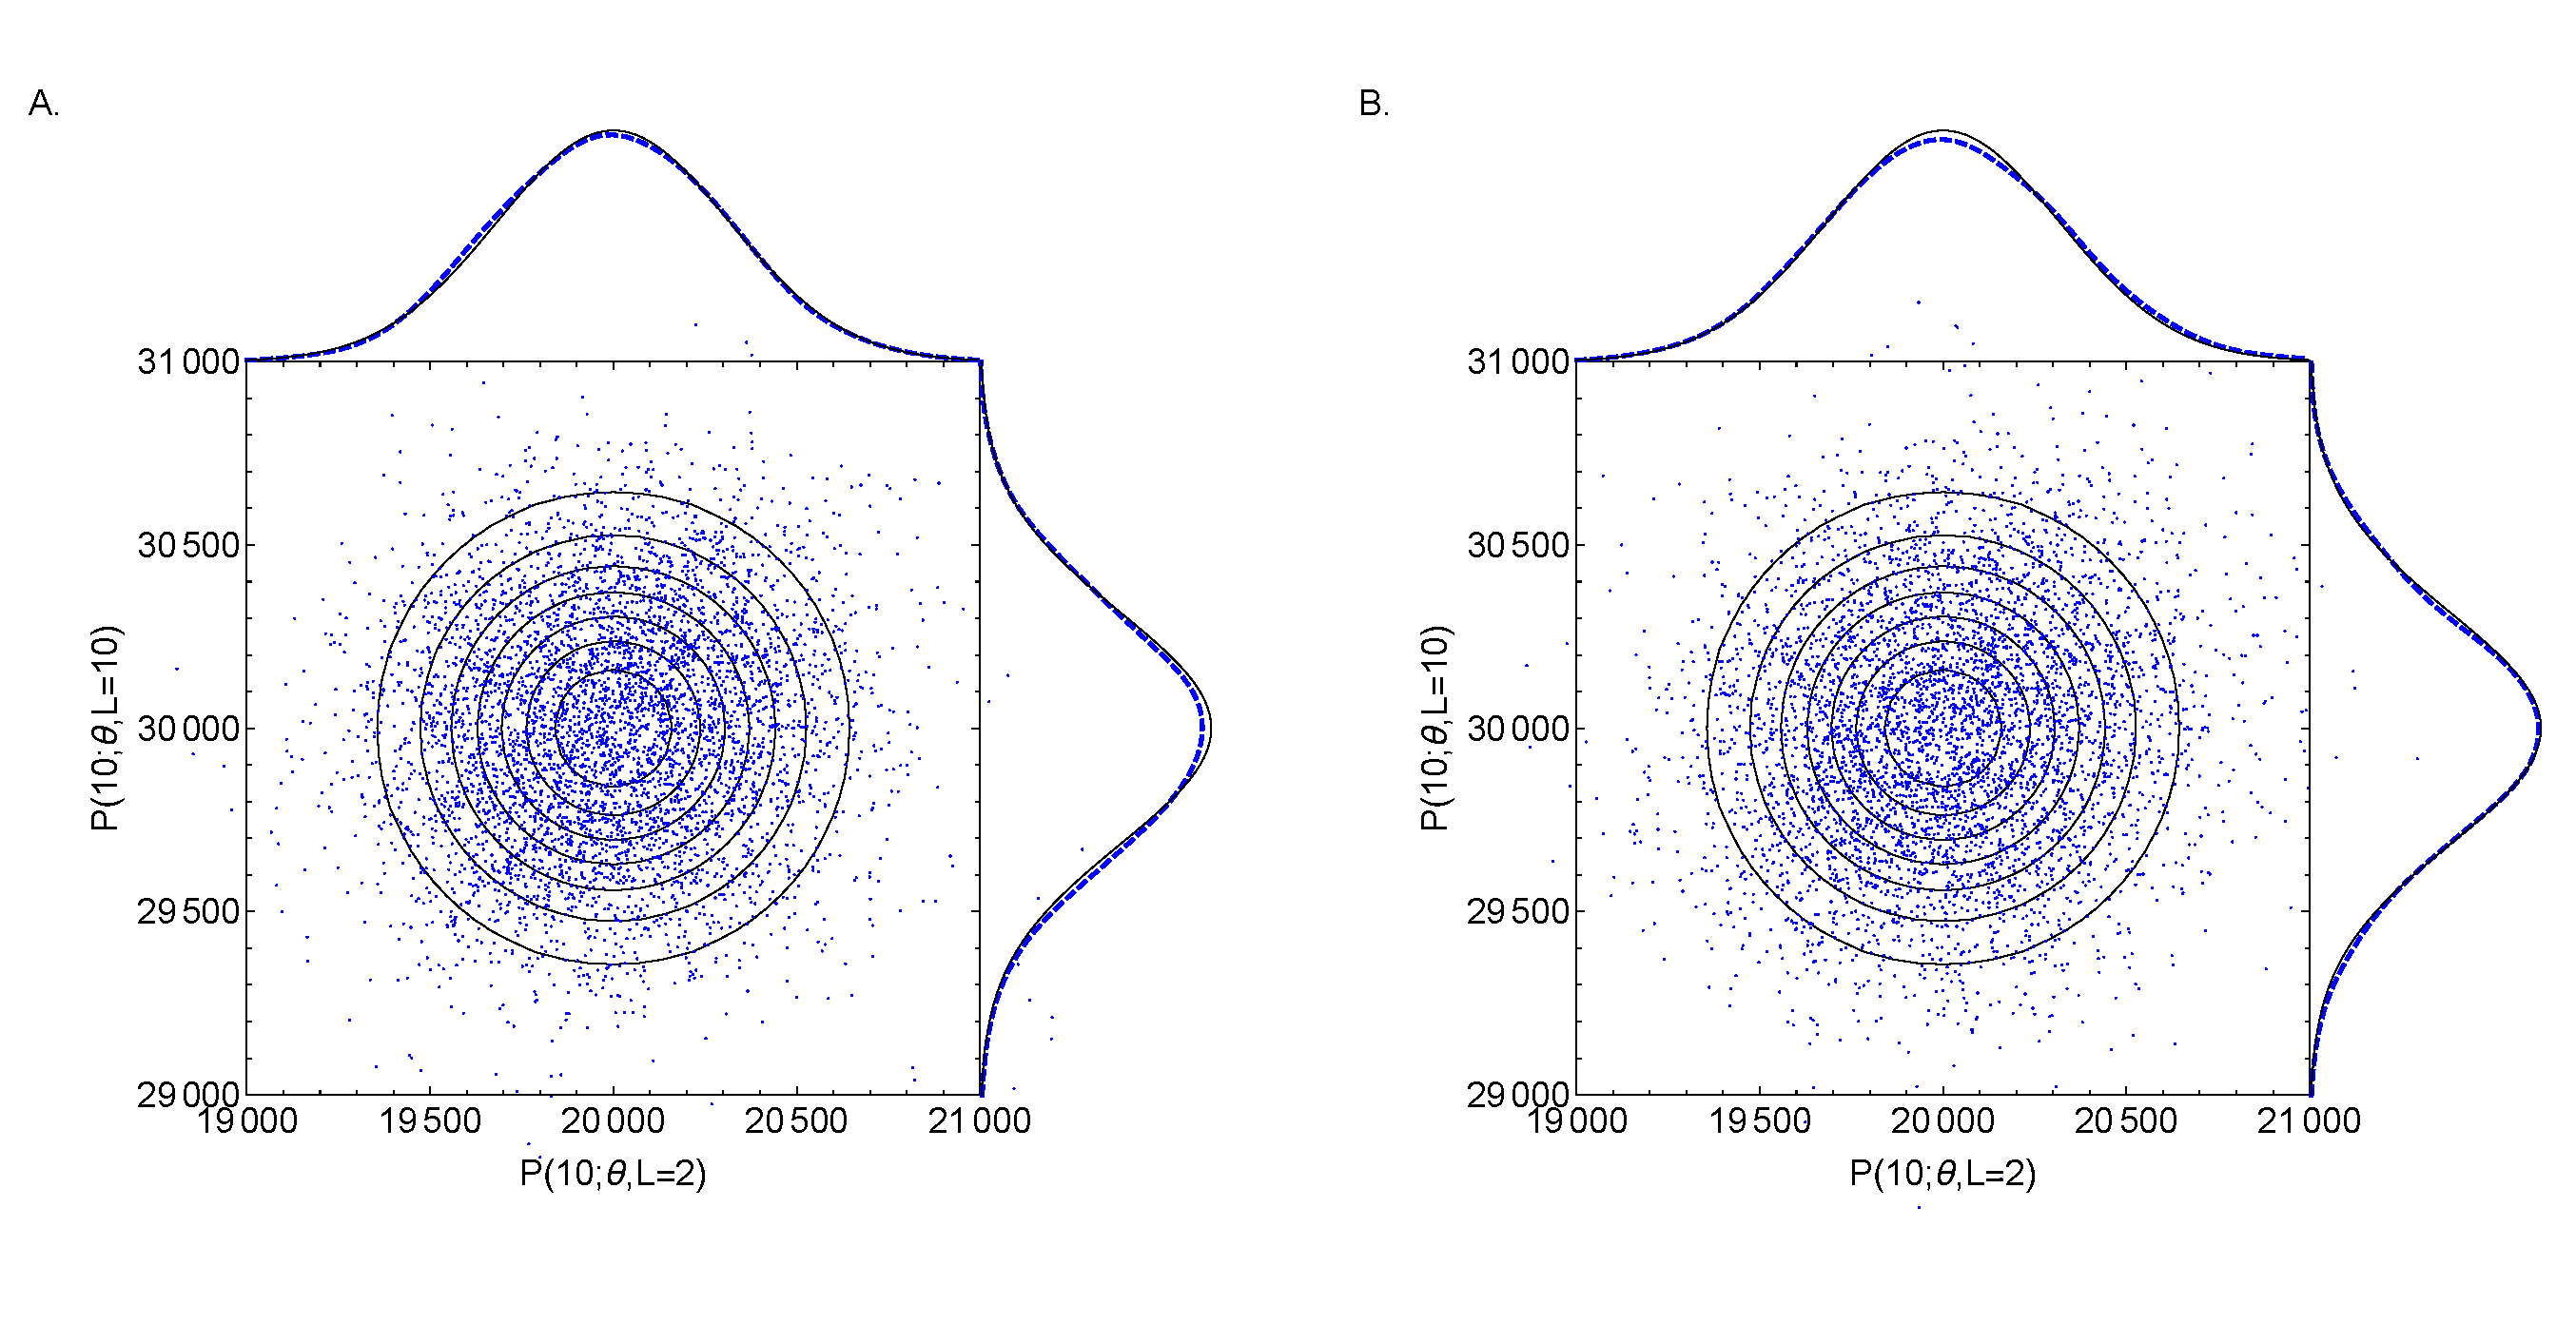
\includegraphics[width=\textwidth]{../figures/growth_factor_outputs.pdf}}
	\caption{\textbf{The target joint output distribution (solid contour lines) and target marginal distributions (solid) versus outputs sampled by CMC (blue dots and dashed lines) for (A) uniform and (B) normal parameter priors.} In the CMC, 100,000 independent samples were used in the ``ContourVolumeEstimator'' step and 10,000 MCMC samples across each of 4 Markov chains were used in the second step, with the first half of the chains discarded as ``warm-up'' \cite{lambert2018Student}. For the reconstructed marginal densities in the plots, we use Mathematica's ``SmoothKernelDistribution'' function specifying bandwidths of 100 with Gaussian kernels \cite{mathematica}.}
	\label{fig:growth_factor_outputs}
\end{figure}

\begin{figure}[H]
	\centerline{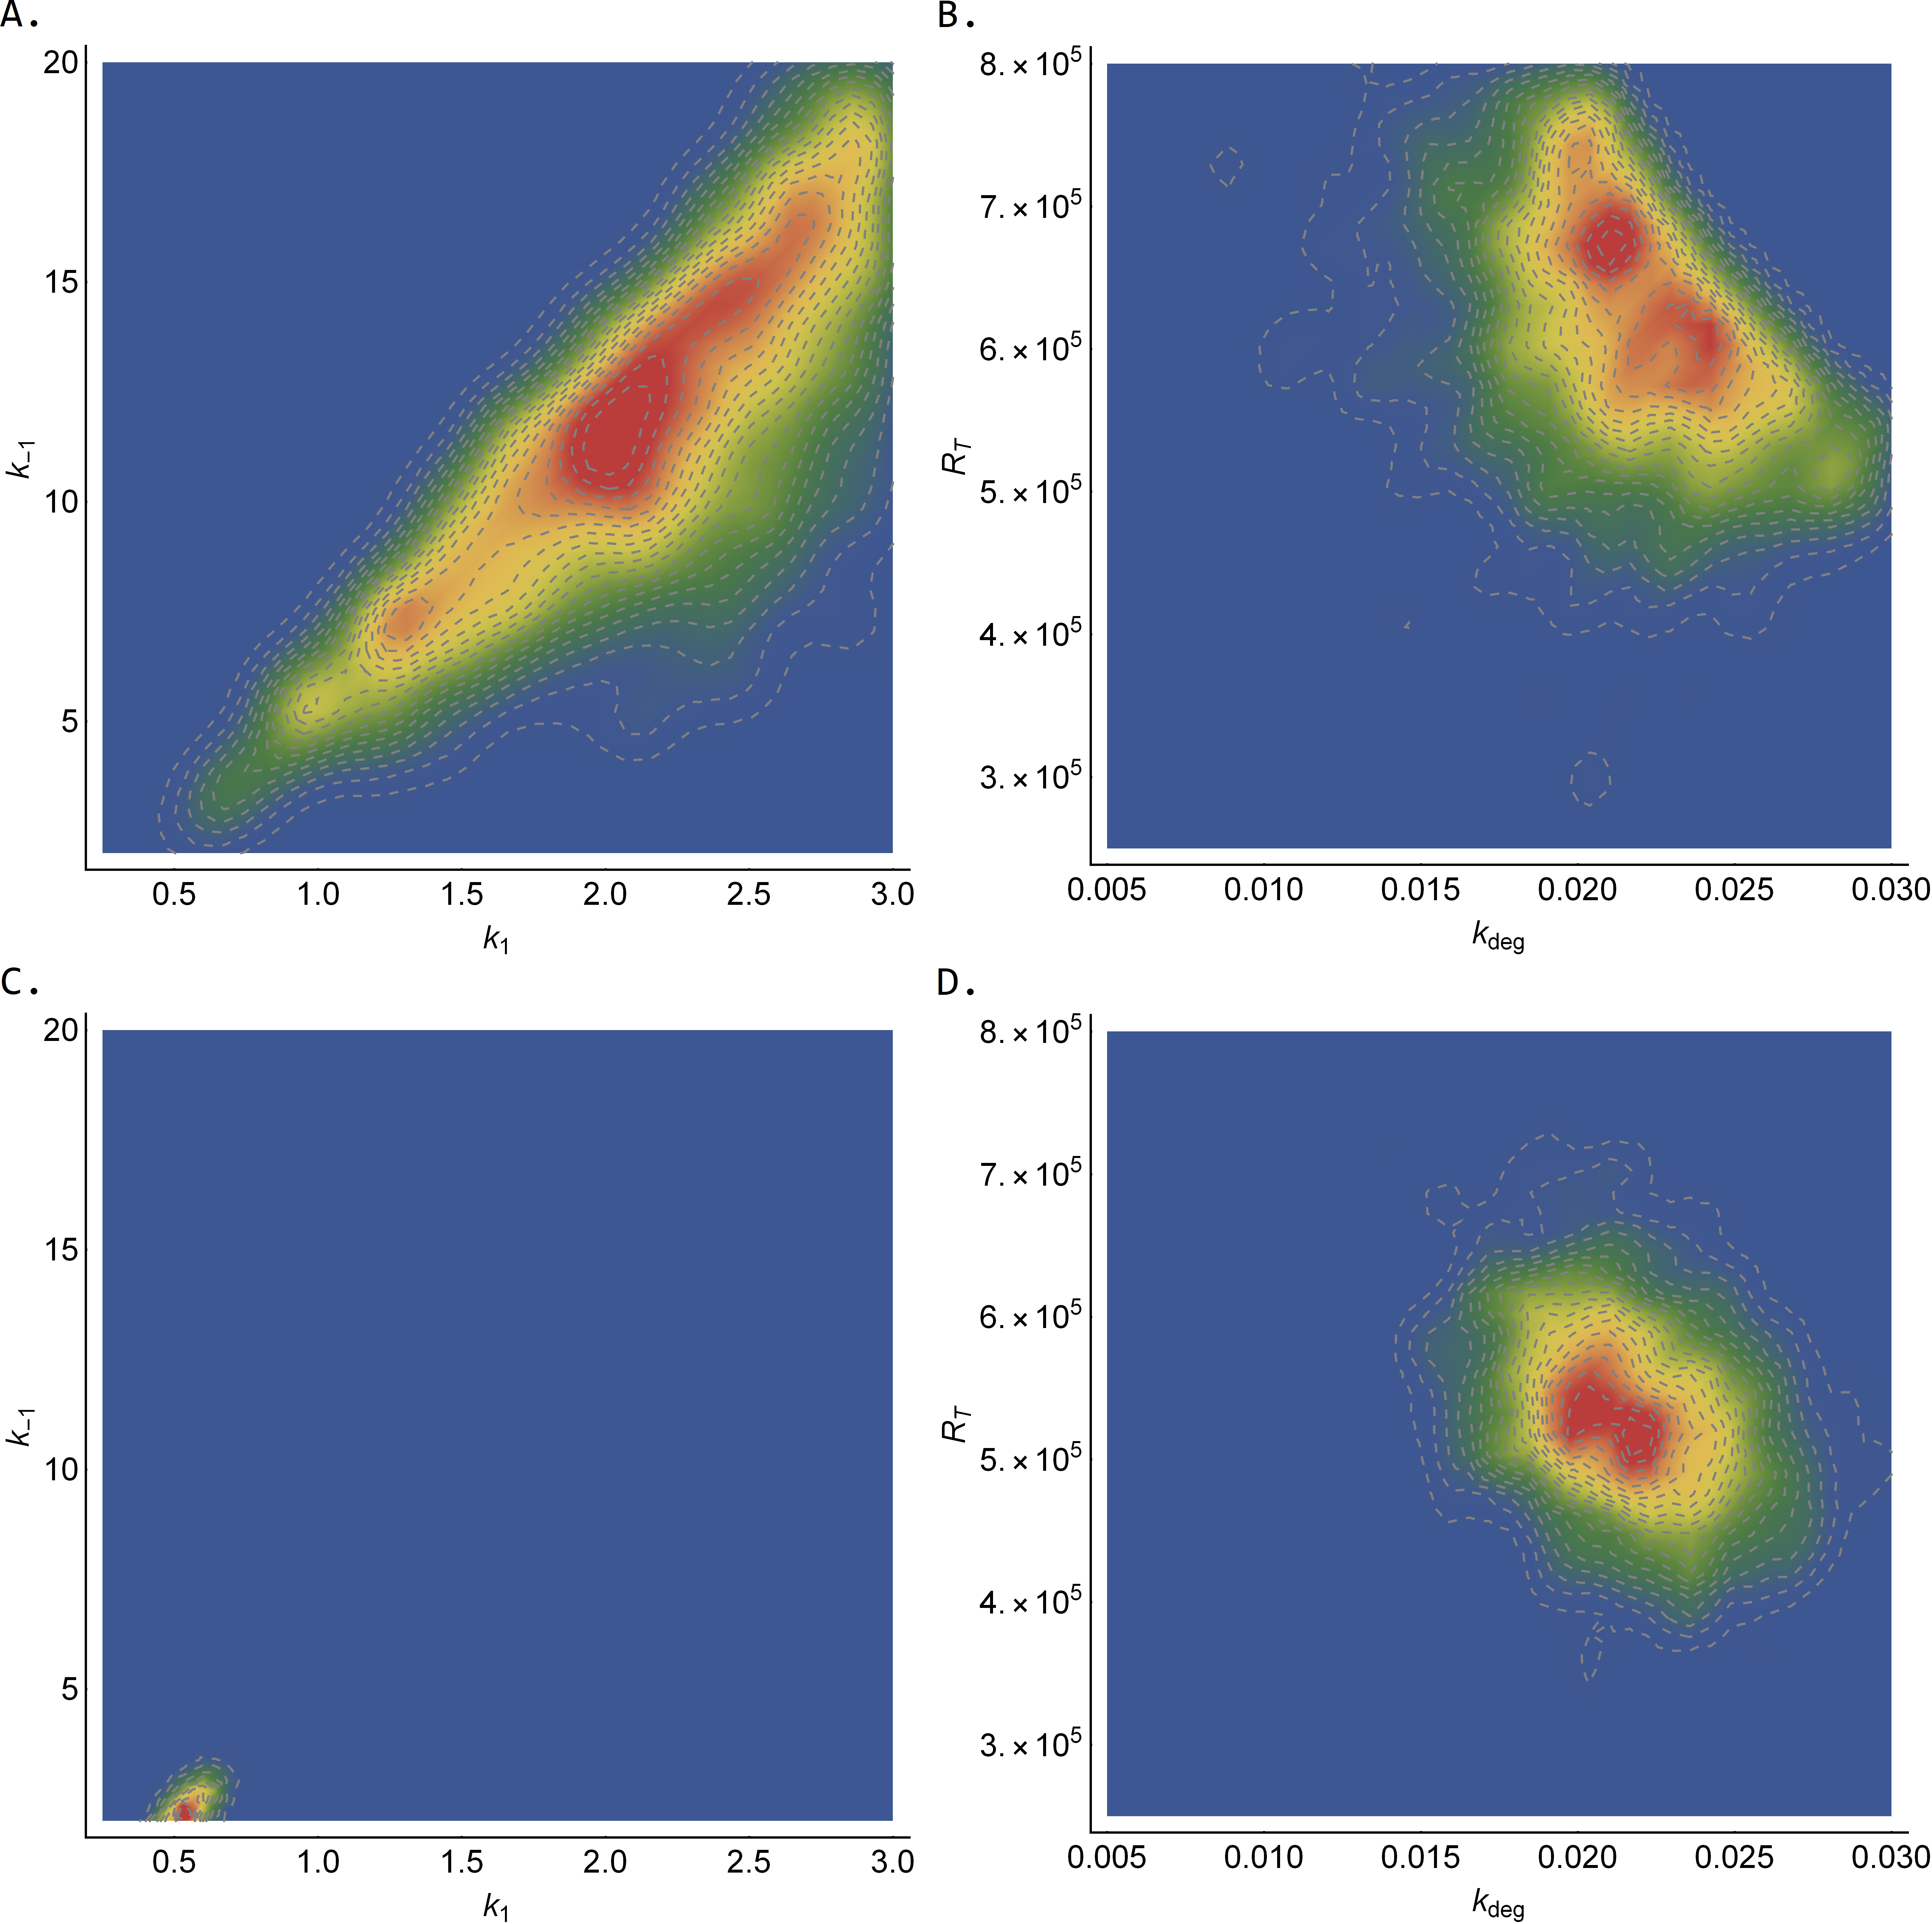
\includegraphics[width=\textwidth]{../figures/growth_factor_inputs.png}}
	\caption{\textbf{The joint distribution of $(k_1,k_{-1})$ for the growth factor model using (A) uniform priors and (B) normal priors.} See Figure \ref{fig:growth_factor_outputs} caption for CMC details and Table \ref{tab:priors} for the priors used.}
	\label{fig:growth_factor_inputs}
\end{figure}

For an unidentified model, there are typically a multitude of possible probability distributions over parameters which map to the same target output distribution. To reduce the space of posterior parameter distributions to one, it is therefore necessary to specify a prior parameter distribution. CMC accommodates the effect of changes to a prior distribution directly, through changes to both the ``ContourVolumeEstimation'' step and the acceptance ratio in the ``MCMC'' step (Algorithm \ref{alg:cmc}), such that the posterior parameter distribution maps to the same output target. We now use CMC to estimate the posterior parameter distribution when changing from uniform to normal priors (prior hyperparameters shown in Table \ref{tab:priors}). As desired, the target output distribution is invariant (Figure \ref{fig:growth_factor_outputs}B) although Figure \ref{fig:growth_factor_inputs}B illustrates that the posterior distribution for $(k_1,k_{-1})$ exhibits substantial change, due to the concentration of the priors used.

\begin{table}
\begin{tabular}{c|ccc|ccc}
	& \multicolumn{3}{c}{Uniform} & \multicolumn{3}{c}{Normal}\\
	Parameter & 2.5\% & 50\% & 97.5\% & 2.5\% & 50\% & 97.5\%\\
	\toprule
	$R_T$ & 441010 & 606440 & 772480 & 408400 & 529560 & 678630 \\
	$k_1$ & 0.89 & 2.16 & 2.95 & 0.39 & 0.54 & 0.70 \\
	$k_{-1}$ & 4.35 & 11.23 & 18.71 & 1.39 & 2.26 & 3.35 \\
	$k_{deg}$ & 0.01 & 0.02 & 0.03 & 0.02 & 0.02 & 0.03 \\
	$k^*_{deg}$ & 0.20 & 0.40 & 0.49 & 0.22 & 0.33 & 0.46 \\
\end{tabular}
\caption{\textbf{Estimated quantiles from CMC samples for the growth factor model with uniform and normal priors.} The particular priors used in each case are given in Table \ref{tab:priors}.}
\label{tab:growth_factor_results}
\end{table}

\subsection{Michaelis-Menten kinetics}
The Michaelis-Menten model of enzyme kinetics (see, for example, \cite{murray2007mathematical}), describes the dynamics of concentrations of an enzyme ($E$), a substrate ($S$), an enzyme-substrate complex ($ES$), and a product ($P$). Specifically,
%
\begin{equation}\label{eq:michaelis_menten}
\begin{aligned}
\frac{dE(t)}{dt}  &= -k_f E(t)S(t) + k_r ES(t) + k_{cat} ES(t), \\
\frac{dS(t)}{dt}  &= -k_f E(t)S(t) + k_r ES(t), \\
\frac{dES(t)}{dt} &= \phantom{-}k_f E(t)S(t) - k_r ES(t) - k_{cat} ES(t), \\
\frac{dP(t)}{dt}  &= \phantom{-}k_{cat} ES(t),
\end{aligned}
\end{equation}
%
with initial conditions
\begin{equation}
E(0) = E_0, \; S(0)=S_0, \; ES(0)=ES_0, \; P(0)=P_0,
\end{equation}
%
where $k_f$ is the rate constant for the forward reaction $E+S\rightarrow ES$, $k_r$ is the rate of the reverse reaction $ES\rightarrow E+S$, and $k_{cat}$ is the catalytic rate at which the product is formed by the reaction $ES\rightarrow E + P$.

When subpopulations of cells, each with distinct dynamics, are thought to exist, determining their characteristics - proportions of overall cell number, likely parameter values, and so on - is often of key interest \cite{hasenauer2011identification,loos2018hierarchical}. Before formal inference occurs, multi-modality of the output distribution may signal the existence of fragmented subpopulations of cells. Here we target the following bimodal bivariate normal distribution,
%
\begin{align}
f(\boldsymbol{x}; \boldsymbol{\mu}_1,\Sigma_1, \boldsymbol{\mu}_2, \Sigma_2) = \frac{1}{2}\left(\mathcal{N}(\boldsymbol{x}; \boldsymbol{\mu}_1,\Sigma_1) + \mathcal{N}(\boldsymbol{x}; \boldsymbol{\mu}_2,\Sigma_2)\right),
\end{align}
%
where $E(2; \boldsymbol{\theta})$ and $S(1; \boldsymbol{\theta})$ corresponds to the solutions of eq. (\ref{eq:michaelis_menten}) for the enzyme and substrate at times $t=2$ and $t=1$, respectively, and $\boldsymbol{\theta}=(k_f,k_r,k_{cat})$. The parameters of the mixture normal output distribution we target are $\boldsymbol{\mu}_1=[2.2, 1.6]'$, $\Sigma_1 = \bigl( \begin{smallmatrix}0.018 & -0.013\\ -0.013 & 0.010\end{smallmatrix}\bigr)$, $\boldsymbol{\mu}_2=[2.8, 1.0]'$ and $\Sigma_2=( \begin{smallmatrix}0.020 & -0.010\\ -0.010 & 0.020\end{smallmatrix}\bigr)$. In what follows, we specify uniform priors on each of the elements of $\boldsymbol{\theta}$ (see Table \ref{tab:priors}).


Using a modest number of samples in each step, CMC was able to well-replicate the output target distribution (Figure \ref{fig:mm_bimodal_inputs_outputs}A). Without specifying \textit{a priori} information on the subpopulations of cells, two distinct clusters of cells emerged from application of CMC (orange and blue dots in Figure \ref{fig:mm_bimodal_inputs_outputs}B), each corresponding to distinct modes of the output distribution (corresponding coloured dots in Figure \ref{fig:mm_bimodal_inputs_outputs}A). It is worth noting however that the issues inherent with MCMC sampling of multimodal distributions similarly apply here and so, whilst here adaptive MCMC \cite{johnstone2016uncertainty} sufficed for exploration of the posterior surface, it may be necessary to use MCMC methods known to be robust to such geometries (for example, population MCMC \cite{jasra2007population}). 

\begin{figure}[H]
	\centerline{\includegraphics[width=\textwidth]{../figures/mm_bimodal_inputs_outputs.pdf}}
	\caption{\textbf{(A) bimodal target distribution (solid contour lines) versus output samples (dots) for the Michaelis-Menten model and (B) posterior parameter samples (dots).} The orange (blue) dots in A were generated by the orange (blue) parameter samples in B. See Figure \ref{fig:growth_factor_outputs} caption for CMC details. For the reconstructed marginal densities in the plots, we use Mathematica's ``SmoothKernelDistribution'' function with Gaussian kernels with (A) default bandwidths and (B) bandwidths of 0.3 (horizontal axis) and 0.03 (vertical axis) \cite{mathematica}. The clusters were identified by applying Mathematica's ``ClusteringComponents'' function to the pairs of parameter samples displayed in B \cite{mathematica}.}
	\label{fig:mm_bimodal_inputs_outputs}
\end{figure}


Target a bimodal target then a four-dimensional covariance target.

\subsection{TNF signalling pathway}
Target a bimodal target. Look in tnf Mathematica file as have already made some nice figures.

Show that varying an input producing an output does not result in recapitulating the input.


\section{Discussion}
\label{sec:discussion}
To do:

Make clear that inference is not circular here typically, since we are in an unidentified region.

When struggling to target a given distribution using this method, this indicates a) the contour estimates are not refined enough and b) that the generating model (without measurement uncertainty) is unable to recapitulate the target.


\section{Author contributions}
BL, DJG and SJT conceived the study. BL carried out the analysis. All authors helped to write and edit the manuscript.


\nolinenumbers

\bibliographystyle{unsrt}
\bibliography{Bayes}
\end{document}
